\def\year{2021}\relax
%File: formatting-instructions-latex-2021.tex
%release 2021.1
\documentclass[letterpaper]{article} % DO NOT CHANGE THIS
\usepackage{aaai21}  % DO NOT CHANGE THIS
\usepackage[switch]{lineno}  %TEMPORARY FOR REVIEW VERSION ONLY
\usepackage{times}  % DO NOT CHANGE THIS
\usepackage{helvet} % DO NOT CHANGE THIS
\usepackage{courier}  % DO NOT CHANGE THIS
\usepackage[hyphens]{url}  % DO NOT CHANGE THIS
\usepackage{graphicx} % DO NOT CHANGE THIS
\urlstyle{rm} % DO NOT CHANGE THIS
\def\UrlFont{\rm}  % DO NOT CHANGE THIS
\usepackage{natbib}  % DO NOT CHANGE THIS AND DO NOT ADD ANY OPTIONS TO IT
\usepackage{caption} % DO NOT CHANGE THIS AND DO NOT ADD ANY OPTIONS TO IT
\frenchspacing  % DO NOT CHANGE THIS
\setlength{\pdfpagewidth}{8.5in}  % DO NOT CHANGE THIS
\setlength{\pdfpageheight}{11in}  % DO NOT CHANGE THIS
\usepackage{lipsum}

\usepackage[ruled,vlined,linesnumbered]{algorithm2e} % ADDED BY RONI
\usepackage{booktabs} % ADDED BY RONI

%\nocopyright
%PDF Info Is REQUIRED.
% For /Author, add all authors within the parentheses, separated by commas. No accents or commands.
% For /Title, add Title in Mixed Case. No accents or commands. Retain the parentheses.
\pdfinfo{
/Title (Improving Continuous-time Conflict Based Search)
/Author (Us)
/TemplateVersion (2021.1)
} %Leave this
% /Title ()
% Put your actual complete title (no codes, scripts, shortcuts, or LaTeX commands) within the parentheses in mixed case
% Leave the space between \Title and the beginning parenthesis alone
% /Author ()
% Put your actual complete list of authors (no codes, scripts, shortcuts, or LaTeX commands) within the parentheses in mixed case.
% Each author should be only by a comma. If the name contains accents, remove them. If there are any LaTeX commands,
% remove them.

% DISALLOWED PACKAGES
% \usepackage{authblk} -- This package is specifically forbidden
% \usepackage{balance} -- This package is specifically forbidden
% \usepackage{color (if used in text)
% \usepackage{CJK} -- This package is specifically forbidden
% \usepackage{float} -- This package is specifically forbidden
% \usepackage{flushend} -- This package is specifically forbidden
% \usepackage{fontenc} -- This package is specifically forbidden
% \usepackage{fullpage} -- This package is specifically forbidden
% \usepackage{geometry} -- This package is specifically forbidden
% \usepackage{grffile} -- This package is specifically forbidden
% \usepackage{hyperref} -- This package is specifically forbidden
% \usepackage{navigator} -- This package is specifically forbidden
% (or any other package that embeds links such as navigator or hyperref)
% \indentfirst} -- This package is specifically forbidden
% \layout} -- This package is specifically forbidden
% \multicol} -- This package is specifically forbidden
% \nameref} -- This package is specifically forbidden
% \usepackage{savetrees} -- This package is specifically forbidden
% \usepackage{setspace} -- This package is specifically forbidden
% \usepackage{stfloats} -- This package is specifically forbidden
% \usepackage{tabu} -- This package is specifically forbidden
% \usepackage{titlesec} -- This package is specifically forbidden
% \usepackage{tocbibind} -- This package is specifically forbidden
% \usepackage{ulem} -- This package is specifically forbidden
% \usepackage{wrapfig} -- This package is specifically forbidden
% DISALLOWED COMMANDS
% \nocopyright -- Your paper will not be published if you use this command
% \addtolength -- This command may not be used
% \balance -- This command may not be used
% \baselinestretch -- Your paper will not be published if you use this command
% \clearpage -- No page breaks of any kind may be used for the final version of your paper
% \columnsep -- This command may not be used
% \newpage -- No page breaks of any kind may be used for the final version of your paper
% \pagebreak -- No page breaks of any kind may be used for the final version of your paperr
% \pagestyle -- This command may not be used
% \tiny -- This is not an acceptable font size.
% \vspace{- -- No negative value may be used in proximity of a caption, figure, table, section, subsection, subsubsection, or reference
% \vskip{- -- No negative value may be used to alter spacing above or below a caption, figure, table, section, subsection, subsubsection, or reference

\setcounter{secnumdepth}{0} %May be changed to 1 or 2 if section numbers are desired.

% The file aaai21.sty is the style file for AAAI Press
% proceedings, working notes, and technical reports.
%

%=====================================
%The following commands were added by Konstantin
%to support acronyms and in-text comments
%=====================================
\usepackage{amsmath}
\usepackage{amssymb}
%
% Add comments in the text
%
\usepackage{ifthen}
\usepackage{xcolor}
\newboolean{showcomments}
% \setboolean{showcomments}{true}
\setboolean{showcomments}{false}

\ifthenelse{\boolean{showcomments}}
  {\newcommand{\nb}[3]{
  {\color{#2}\small\fbox{\bfseries\sffamily\scriptsize#1}}
  {\color{#2}\sffamily\small$\triangleright~$\textit{\small #3}$~\triangleleft$}
  }
  }
  {\newcommand{\nb}[3]{}
  }

\newcommand\konstantin[1]{\nb{\textbf{Konstantin:}}{red}{#1}}
\newcommand\roni[1]{\nb{\textbf{Roni:}}{orange}{#1}}
\newcommand\anton[1]{\nb{\textbf{Anton:}}{cyan}{#1}}
\newcommand\eli[1]{\nb{\textbf{Eli:}}{green}{#1}}

\usepackage{acronym}
\usepackage{xspace}
\acrodef{SOC}{sum of costs}
\acrodef{SIPP}{Safe interval path planning}
\acrodef{CBS}{Conflict-based search}
\acrodef{CCBS}{Continuous-time conflict-based search}
\acrodef{CCBS-DS}{Continuous-time conflict-based search with disjoint splitting}
\acrodef{ICBS}{Improved conflict-based search}
\acrodef{MAPF}{Multi-Agent Pathfinding}
\acrodef{ICTS}{Increasing Cost Tree Search}
\acrodef{MCCBS}{Multi-Constraint CBS}
\acrodef{CT}{Constraint Tree}
\acrodef{PC}{Prioritizing Conflicts}
\acrodef{DS}{Disjoint Splitting}



\newcommand{\cbs}{\ac{CBS}\xspace}
\newcommand{\icbs}{\ac{ICBS}\xspace}
\newcommand{\ccbs}{\ac{CCBS}\xspace}
\newcommand{\ccbsds}{\ac{CCBS-DS}\xspace}
\newcommand{\cbsh}{{CBS-H}\xspace}
\newcommand{\cbsds}{{CBS-DS}\xspace}
\newcommand{\ct}{\ac{CT}\xspace}
\newcommand{\sipp}{\ac{SIPP}\xspace}
\newcommand{\soc}{\ac{SOC}\xspace}
\newcommand{\astar}{A$^*$\xspace}
\newcommand{\mapfr}{{MAPF}$_R$\xspace}
\newcommand{\mapf}{\ac{MAPF}\xspace}
\newcommand{\const}{\textit{constraints}\xspace}
\newcommand{\safe}{\textit{Safe}\xspace}
\newcommand{\pc}{\ac{PC}\xspace}
\newcommand{\ds}{\ac{DS}\xspace}
\newcommand{\open}{\textit{OPEN}\xspace}


\newtheorem{definition}{Definition}
\newtheorem{lemma}{Lemma}
\newtheorem{theorem}{Theorem}
%=====================================
%end of the commands added by Konstantin
%=====================================

% Title

% Your title must be in mixed case, not sentence case.
% That means all verbs (including short verbs like be, is, using,and go),
% nouns, adverbs, adjectives should be capitalized, including both words in hyphenated terms, while
% articles, conjunctions, and prepositions are lower case unless they
% directly follow a colon or long dash

\title{Improving Continuous-time Conflict Based Search}
\author{
Submission \#6374
}
\affiliations{

}
\iffalse
%Example, Single Author, ->> remove \iffalse,\fi and place them surrounding AAAI title to use it
\title{My Publication Title --- Single Author}
\author {
    % Author
    Author Name \\
}

\affiliations{
    Affiliation \\
    Affiliation Line 2 \\
    name@example.com
}
\fi

\iffalse
%Example, Multiple Authors, ->> remove \iffalse,\fi and place them surrounding AAAI title to use it
\title{My Publication Title --- Multiple Authors}
\author {
    % Authors

        First Author Name,\textsuperscript{\rm 1}
        Second Author Name, \textsuperscript{\rm 2}
        Third Author Name \textsuperscript{\rm 1} \\
}
\affiliations {
    % Affiliations
    \textsuperscript{\rm 1} Affiliation 1 \\
    \textsuperscript{\rm 2} Affiliation 2 \\
    firstAuthor@affiliation1.com, secondAuthor@affilation2.com, thirdAuthor@affiliation1.com
}
\fi
\begin{document}

\maketitle

\linenumbers  %TEMPORARY FOR REVIEW VERSION

\begin{abstract}
%KONSTANTIN: I purposefully did not use acronym commands in abstract
Conflict-Based Search (CBS) is a powerful algorithmic framework for optimally solving classical multi-agent path finding (MAPF) problems, where time is discretized into the time steps. 
%If time is not discretized, the number of possible wait actions is uncountable. 
Continuous-time CBS (CCBS) is a recently proposed version of CBS that guarantees optimal solutions without the need to discretize time. 
However, the  scalability of CCBS is limited because it does not include any known improvements of CBS. 
In this paper, we begin to close this gap and explore how to adapt successful CBS improvements, namely, prioritizing conflicts (PC), disjoint splitting (DS), and high-level heuristics, to the continuous time setting of CCBS. 
%domain is not trivial as requires careful reasoning over the time intervals and the ways different time intervals interfere. 
These adaptions are not trivial, and require careful handling of different types of constraints, applying a generalized version of the \acf{SIPP} algorithm, and extending the notion of cardinal conflicts.  
% Moreover, the adaptions are applicable to other CBS-based algorithms that address have non-unit action costs. 
We evaluate the effect of the suggested enhancements by running experiments both on general graphs and $2^k$-neighborhood grids. 
CCBS with these improvements significantly outperforms vanilla CCBS, 
solving problems with almost twice as many agents in some cases and 
pushing the limits of multi-agent path finding in continuous-time domains. 

%with 50 agents more in some cases. The overall amount of solved instances on the evaluated scenarios on grids and roadmaps has increased on 47.6\% - from 2624 to 3873. While vanilla CCBS algorithm can optimally solve problems with only 11.6 agents on roadmaps and 25.4 agents on grids in average, the most advanced version of CCBS increases these values to 18.4 and 34.25 respectively.
%The most advanced version of the improved CCBS (the one that simultaneously incorporates DS, PC, H) significantly outperforms vanilla CCBS pushing the limits of multi-agent path finding in continuous-time domains. The overall amount of solved instances on the evaluated scenarios on grids and roadmaps has increased on 47.6\% - from 2624 to 3873. While vanilla CCBS algorithm can optimally solve problems with only 11.6 agents on roadmaps and 25.4 agents on grids in average, the most advanced version of CCBS increases these values to 18.4 and 34.25 respectively.
%\roni{Can you put some show-off numbers, e.g., something like ``Is able to go from optimally solving problems with X agents to Y agents''}
% \roni{Maybe better to put numbers that show the limit of the benefit we've seen, i.e., something like ``The Improved CBS can solve in some cases problems with X times more agents than vanilla CCBS''}
% \roni{Also, we need to shorten the abstract}


% Conflict-based search (CBS) is a powerful algorithm for optimally solving multi-agent path finding problems when time is discretized into the time steps and CCBS is an adaptation of CBS for continuous-time domains, in which the number of wait actions is uncountable. It is known that the performance of CBS can be drastically enhanced by techniques such as prioritizing conflicts (PC), disjoint splitting (DS), high-level heuristics (H) etc, however CCBS does not incorporate them. In this paper we present the pathways to utilizing PC, DS and H in CCBS. Adaptation of these techniques to continuous time domain is not trivial as requires careful reasoning over the time intervals and the ways different time intervals interfere. We present detailed explanation on this. We evaluate the effect of the suggested enhancements by running experiments both on general graphs and 8-connected grids. The most advanced version of the improved CCBS (the one that simultaneously incorporates DS, PC, H) significantly outperforms vanilla CCBS pushing the limits of multi-agent path finding in continuous-time domains.

\end{abstract}

\section{Introduction}

% What is MAPF
\acf{MAPF} is the problem of finding paths for $n>1$ agents in a graph such that 
each agent reaches its desired goal vertex and the agents do not collide with each other while moving along these paths. 
Many real-world applications require solving variants of \mapf, 
including managing aircraft-towing vehicles \cite{MorrisPLMMKK16}, video game characters \cite{Silver05}, office robots \cite{VelosoBCR15}, and warehouse robots \cite{WurmanDM07}. 
Finding an optimal solution to a \mapf problem for common objective functions is NP-Hard~\cite{surynek2010optimization,yu2013structure}, 
but modern optimal \mapf algorithms can scale to problems with over a hundred agents~\cite{sharon2015conflict,BoyarskiFSSTBS15,felner2018adding,BCP,lazy-cbs,SurynekFSB16}.

% Classical MAPF scales, but MAPFR is much harder. 
However, such scaling has been demonstrated mostly on the classical version of the \mapf problem~\cite{stern2019multi}, which embodies several simplifying assumptions such as all actions have the same duration and time is discretized into time steps. \mapfr~\cite{walker2018extended} is a generalization of the classical \mapf problem in which actions' durations are non-uniform, agents have geometric shapes that must be considered, and time is continuous, that is, it is not discretized into time steps. 
Handling continuous time in \mapfr is especially challenging because it implies an agent may wait in a location for an arbitrary amount of time, i.e., the number of \emph{wait actions} is infinite.  

% Others and CCBS
Several recently proposed algorithms address the \mapfr problem or limited variants of it, such as Extended ICTS (E-ICTS)~\cite{walker2018extended}, CBS with Continuous Time (CBS-CT)~\cite{cohen2019optimal}, and \ccbs~\cite{andreychuk2019multi}. A direct comparison between these algorithms is problematic as they make different underlying assumptions. 
%However limited comparison did not reveal one approach to dominate the others~\cite{andreychuk2019multi}, and none has been able to scale to more than 50 agents in reasonable time. %30 seconds. 
However, none has been able to scale to more than 50 agents in reasonable time. %30 seconds. 

% Our focus
In this work, we propose several improvements to \ccbs that allow it to solve \mapfr problems with significantly more agents in some cases. 
% focus on \ccbs, which  the most general definition of \mapfr, and suggest several improvements that allow it to solve \mapfr problems with significantly more agents. 
\ccbs is based on the \cbs algorithm for classical \mapf, and the improvements we propose for \ccbs are based on known improvements of \cbs, namely \ds, \pc, and high-level heuristics. 
Adapting the \ds technique to the continuous-time setting of \mapfr requires solving a single-agent pathfinding problem with temporally-constrained action landmarks~\cite{karpas2009cost}. 
We show how to efficiently solve this pathfinding problem in our context by applying a generalized version of the \sipp algorithm~\cite{phillips2011sipp}. 
A naive applying of \pc to \ccbs is shown to be ineffective, and we propose an adapted version of \pc that can cut the number of expanded nodes significantly. 
The third \ccbs improvement we propose is an admissible heuristic function for \ccbs that require only a negligable amount of overhead when applied together with the \pc technique. 


% Results
Finally, we evaluate the impact of these improvements individually and collectively on several benchmarks, including both roadmaps and grids. 
The results show that the number of \mapfr instances solved by \ccbs with all the proposed improvements compared to vanilla CCBS
has increased by 47.6\% --- from 2,624 to 3,873. 
In some cases, it can even solve problems with approximately twice the number of agents compared to vanilla CCBS. 
%,  algorithm can optimally solve problems with only 11.6 agents on roadmaps and 25.4 agents on grids in average, the most advanced version of CCBS increases these values to 18.4 and 34.25 respectively.
%The most advanced version of the improved CCBS (the one that simultaneously incorporates DS, PC, H) significantly outperforms vanilla CCBS pushing the limits of multi-agent path finding in continuous-time domains. The overall amount of solved instances on the evaluated scenarios on grids and roadmaps has increased on 47.6\% - from 2624 to 3873. While vanilla CCBS algorithm can optimally solve problems with only 11.6 agents on roadmaps and 25.4 agents on grids in average, the most advanced version of CCBS increases these values to 18.4 and 34.25 respectively.
%\roni{Can you put some show-off numbers, e.g., something like ``Is able to go from optimally solving problems with X agents to Y agents''}
% \roni{Maybe better to put numbers that show the limit of the benefit we've seen, i.e., something like ``The Improved CBS can solve in some cases problems with X times more agents than vanilla CCBS''}




% Finally, we present a heuristics in some case and we propose a 
% . In some cases, adapting these improvement is simple, but

% The first improvement we propose is a continuous-time version of the \ds technique, which was previously described for classical \mapf. 


% While these algorithms guarantee some form of optimality, they fail to scale beyond 
% Neither of these however is able to solve optimally problems with 
% Recently proposed \mapf Different algorithm 
% \ccbs is a recently proposed optimal \mapf algorithm for solving \mapfr problems, where time is not 

% and time is discretized, and agents d

% However, most of the earlier work assumed the time it takes an agent to traverse an edge is fixed and known a priori. 
% In reality, exogenous events may cause the edge traversal time to be non-deterministic. 
% One approach to address this is to gather statistics over these exogenous events and reason about them~\cite{wagner2017path,atzmon2020probabilistic,0001KK17}. %\dor{What paper does Sven have that should be cited here? Is it "Multi-Agent Path Finding with Delay Probabilities"?}
% However, gathering sufficiently accurate statistics of exogenous events is often difficult. 
% For example, in many automated warehouses, humans are responsible for packing items into boxes and the robots move the packages.
% The time it takes a human to pack a box may depend on many factors, such as the number of items in the box, their weight, and the human's fatigue. Creating an accurate statistical model for the packing time is a challenging problem on its own. 
% In this work, we consider weaker knowledge about such exogenous events, in the form of upper and lower bounds.\footnote{We show a way to obtain such bounds from observations in Section~\ref{sec:discussion}.} That is, we consider the case where each edge is associated with a time range that bounds the duration it takes an agent to traverse it. 
% This form of uncertainty poses a challenge to current MAPF solvers, especially if one wants to find a \emph{safe} solution. A solution is safe if it is guaranteed that when executing it there will not be any collision.\footnote{This is also known as a \emph{strong} solution~\cite{CimattiDMRS18}.} %
% We call the problem of finding a safe solution in this setting, the Multi-Agent Pathfinding with Time Uncertainty (\mapftu) problem. 



% Classical MAPF is very abstract, MAPF$_R$ is an important generalization


% CCBS recently proposed for solving MAPFR optimality. Big benefit: no need for discretization. 
% Challenge: based on basic CBS, so scalability is limited. 

% CBS has many improvements, but how to apply them in the MAPFR scenario.


% Here we report on three such improvements and show they have a huge benefits. 
% Doing this is not trivial and require changes to standard improvements. 


% IMPORTANT: Mention here already how much we improve, to excite the researcher.


\section{Background and Problem Statement}

%In this work we are interested in solving the \mapfr problem optimally~\cite{walker2018extended}. 
In a \mapfr problem~\cite{walker2018extended}, the agents are confined to a weighted graph $G=(V, E)$ whose vertices ($V$) correspond to locations in some metric space, e.g. $\mathbb{R}^2$ in a Euclidean space, and edges ($E$) correspond to possible transitions between these location. 
%In this work, we assume that when moving from one location to the other an agent follows a straight line segment embedded in $\mathbb{R}^2$ connecting the two locations. \roni{I don't think we are assuming this anywhere except in our experiments. All other theory holds regardless. So, I'd move this to the experiments}
Each agent $i$ is initially located at vertex $s_i\in V$ and aims to reach vertex $g_i\in V$. 
When at a vertex, an agent can either perform a \emph{move} action or a \emph{wait} action. 
A move action means moving the agent along an edge. 
% For the sake of simplicity, we assume disk-shaped agents and define the \emph{location} of the agent as the center of this shape. % in this work. \roni{This is already said in the experimental results. No need to say this twice. If you add it here, then you should remove it there.}
We assume that the agent moves in a constant velocity and inertial effects are neglected. 
The duration of a move action is the weight of its respective edge. 
A wait action means the agents stays in its current location for some duration. 
The duration of a wait action can be any positive real value. Since we do not discretize time, the set of possbile wait actions is uncountable. 
%Thus, the set of wait actions is uncountable and the timeline is continuous. \roni{What do you mean by timeline here? maybe just say ``the set of wait actions is uncountable'' without the timeline bit.}

A \emph{timed action} is a pair $(a_i, t_i)$ representing that action $a_i$ (either move or wait) starts at time $t_i$. 
A \emph{plan} for an agent is a sequence of timed actions such that executing this sequence of timed actions moves the agent from its initial location to its goal location. 
The cost of a plan is the sum of the durations of its constituent actions. 
We assume that after finishing the plan the agent does not disappear but rather stays at the last vertex forever, but this ``dummy'' wait action does not add up to the cost of the plan.\footnote{This assumption is common in the MAPF literature.}

The plans of two agents are said to be \emph{conflict free} if the agents following them never collide, i.e. their \emph{shapes} never overlap. 
A \emph{joint plan} is a a set of plans, one per each agent. 
A \emph{solution} to a \mapfr problem is joint plan whose constituent plans are pairwise conflict-free. 
The cost of a solution is its \soc, i.e., the sum of costs of its constituent plans.  
In this work, we are interested in solving \mapfr problems optimally, i.e., finding a  solution with a minimal cost. %that minimizes \soc, which is naturally the sum of costs of the plans comprising the solution.
\ccbs~\cite{andreychuk2019multi} is a \cbs-based algorithm that does so. 
%such an algorithm that is based on the \cbs algorithm.  
For completeness, we provide a brief description of \cbs and \ccbs below. 





\subsection{\acf{CBS}}

% Conflict Based Search (\cbs)
% \konstantin{Copy/paste (with tiny edits) from IJCAI'19 paper on \ccbs.}
\cbs~\cite{sharon2015conflict} is a complete and optimal algorithm for solving classical \mapf problems, i.e., \mapf problems where time is discretized and all actions have the same duration. 
\cbs works by finding plans for each agent separately, detecting \emph{conflicts} between these plans, and resolving them by replanning for the individual agents subject to specific \emph{constraints}.
A \cbs conflict in \cbs is defined by a tuple $(i,j,x,t)$ 
stating that agents $i$ and $j$ have a conflict in location $x$ (either a vertex or an edge) at time $t$. A \cbs constraint is defined by a tuple $(i,x,t)$, which states that agent $i$ cannot occupy $x$ at time $t$. 
To resolve a conflict $(i,j,x,t)$, \cbs replans for agent $i$ or $j$ or both, subject to \cbs constraints $(i,x,t)$ and $(j,x,t)$, respectively. 
To guarantee completeness and optimality, \cbs runs two search algorithms: a low-level search algorithm that finds paths for individual agents subject to a given set of constraints, and a high-level search algorithm that chooses which constraints to impose and which conflicts to resolve. 



% where $i$ and $j$ are agents, $x$ is either a vertex or an edge, and $t$ is a time step. 
% The typical \cbs implementation considers two types of conflicts: a vertex conflict and a swapping conflict. A vertex conflict between plans $\pi_i$ and $\pi_j$ is defined by a tuple $(i,j,v,t)$ and means that according to these plans agents $i$ and $j$ plan to occupy $v$ at the same time step $t$. 
% A swapping conflict is defined by a tuple $(i,j,e,t)$, 
% and means that according to $\pi_i$ and $\pi_j$ both agents
% plan to traverse the edge $e$ at the same time step, from opposite directions. 
% To resolve a conflict $(i,j,x,t)$, \cbs replans either for agent $i$ or $j$ or both, subject to appropriate \cbs constraints. 
% A \cbs constraint is defined by a tuple $(i,x,t)$, which states that agent $i$ cannot occupy $x$ (either vertex or edge) at time $t$. 


% by replanning either for agent $i$ or for agent $j$. To ensure the conflict is avoided, 
% a constrain, subject to the constraint $(i,x,t)$ or $(j,x,y)$ respectively. 
% , \cbs imposes the constraints $($ 
% The conflicts are transformed into constraints as follows.
% A vertex-constraint is defined by a tuple $(i,v,t)$ and means that agent $i$ is prohibited from occupying vertex $v$ at $t$. 
% An edge-constraint is defined similarly by a tuple $(i,e,t)$.


%\roni{Did some wording above, TODO: check if below is too copy and paste}
\paragraph{\cbs: Low-Level Search.}
In the basic \cbs implementation, the low-level search is a search in the state space of vertex-time pairs. 
Expanding a state $(v,t)$ generates states of the form $(v',t+1)$, where $v'$ is either equal to $v$, representing a wait action, or equal to one of the locations adjacent to $v$. 
States generated by actions that violate the given set of \cbs constraints, are pruned. 
\cbs runs \astar on this search space to return the lowest-cost path to the agent's goal that is consistent with the given set of \ac{CBS} constraints, as required.

% The low-level search in \cbs can be any pathfinding algorithm that can find an optimal plan for an agent that is consistent with a given set of \cbs constraints, e.g. \astar that considers the time dimension and identifies the search nodes by tuples $(v,t)$. Expanding a state $(v,t)$ generates states 
% of the form $(v',t+1)$, where $v'$ is either equal to $v$, representing a wait action, 
% or equal to one of the locations adjacent to $v$. States generated by actions that violate the given set of\cbs constraints, are pruned. Indeed, running \astar on this search space will return the lowest-cost path to the agent's goal that is consistent with the given set of \ac{CBS} constraints, as required.


\paragraph{\cbs: High-Level Search.}
The \cbs high-level search is a search in a binary tree called the \ct. 
In the \ct, each node $N$ represents a set of \cbs constraints $N.\const$
%imposed on the agents and 
and a joint plan $N.\Pi$ that is consistent with these constraints. 
% For a \ct node $N$, we denote its constraints and joint plan by $N.\const$ and $N.\Pi$, respectively. 
Generating a node $N$ involves settings its constraints $N.\const$ and running the low-level search to create $N.\Pi$. 
If $N.\Pi$ does not contain any conflict, then $N$ is a goal. 
Expanding a non-goal node $N$ involves choosing a conflict $(i,j,x,t)$ in $N.\Pi$ 
and generating two child nodes $N_i$ and $N_j$. 
Both nodes have the same set of constraints as $N$, plus a new \cbs constraint: $(i,x,t)$ for $N_i$ and $(j,x,t)$ for $N_j$. 
This type of node expansion is referred to as \emph{splitting node $N$ over conflict $(i,j,x,t)$}.
% The joint plan for each node ($N_i.\Pi$ and $N_j.\Pi$) is created by running the low-level search. 
% A \ct node $N$ is generated by setting its constraints ($N.\const$) and 
% computing $N.\Pi$ by running the low-level search.
%solver, which finds a plan for each agent subject to the constraints relevant to it in $N.\const$. 
%Else, one of the \cbs conflicts $(i,j,x,t)$ in $N.\Pi$ is chosen and two new \ct nodes are generated $N_i$ and $N_j$. 
% This is referred to as \emph{splitting the \ct node}. 
The high-level search finds a goal node by searches the \ct in a best-first manner, expanding in every iteration the \ct node $N$ with the lowest-cost joint plan.



\subsection{Continuous-Time Conflict Based Search (CCBS)}

% \ccbs~\cite{andreychuk2019multi} is an algorithm for solving \mapfr

% extension of the \cbs algorithm for continuous-time domains. Recall, that in these domains a duration of an action might be arbitrary, e.g. an agent can wait in a vertex \emph{any} amount of time. 

To consider continuous time, \ccbs reasons over the time intervals rather than the time steps and considers conflicts over timed actions instead of a graph vertex or edge~\cite{andreychuk2019multi}. 
Formally, a \ccbs conflict is a tuple $(a_i, t_i, a_j, t_j)$, where $(a_i, t_i)$ and $(a_j, t_j)$ are timed actions of agents $i$ and $j$, respectively. 
To resolve a \ccbs conflict, \ccbs computes the \emph{unsafe intervals} of the timed actions in the conflict.  
The \emph{unsafe interval} of timed action $(a_i, t_i)$ w.r.t. the timed action $(a_j, t_j)$
is the maximal time interval starting from $t_i$ in which performing $a_i$ creates a conflict with performing $a_j$ at time $t_j$. \roni{Bad connection}
A \ccbs constraint is a tuple $(i, a_i, [t_i, t_i^u))$, indicating that 
agent $i$ cannot perform $a_i$ in the time interval $[t_i, t_i^u)$. 

% \ccbs adds 
% to $N_i$ the constraint that agent $i$ cannot perform $a_i$ in its unsafe interval w.r.t to $a_j$, and adds to $N_j$ the constraint that agent $j$ cannot perform $a_j$ in its unsafe interval w.r.t to $a_i$.


% are the actions of the involved agents and $t_i$, $t_j$ are the time moments they start to perform these actions according to their respective individual plans.
% As our work is based on \cbs framework we start with providing a relevant background.
% \subsection{CCBS}
% \konstantin{To Roni: please check/modify the content of this section.}
% \ccbs~\cite{andreychuk2019multi} is an extension of \cbs for continuous-time domains. Recall, that in these domains a duration of an action might be arbitrary, e.g. an agent can wait in a vertex \emph{any} amount of time. To handle this \ccbs involves reasoning over the time intervals rather than the time steps. Moreover, \ccbs utilizes a different notion of a conflict. Unlike \ccbs that defines a conflict w.r.t. a single graph node or an edge, \ccbs defines it w.r.t. two different actions of two conflicting agent plans. Formally, a \ccbs conflict is a tuple $(a_i, t_i, a_j, t_j)$, where $a_i$, $a_j$ are the actions of the involved agents and $t_i$, $t_j$ are the time moments they start to perform these actions according to their respective individual plans.

% \subsubsection{\ccbs: Low-Level Search}
The low-level planner of \ccbs is an adaptation of the \sipp algorithm~\cite{phillips2011sipp}. 
\sipp was originally designed to find time-optimal paths for an agent moving among the dynamic obstacles with known trajectories. 
\sipp runs a heuristic search in the state-space of $(v, [t, t'])$ tuples, where $v$ is the graph vertex and $[t, t']$ is a \emph{safe interval} of $v$, i.e. a maximal contiguous time interval in which an agent can stay or arrive at $v$ without colliding with a moving obstacle. As numerous obstacles may pass through $v$ there can exist numerous search nodes corresponding to the same graph vertex but different time intervals in the \sipp search tree. 

The \ccbs low-level search is based on \sipp except for how it handles the given \ccbs constraints. 
Instead of dynamic obstacles, the low-level \ccbs computes safe intervals for each vertex $v$ with respect to the \ccbs constraints imposed over wait actions at $v$. 
Initially, vertex $v$ has a single safe interval $[0, \infty)$. 
Then, for every \ccbs constraint $(i, a_i, [t_i, t_i^u))$ 
where $a_i$ is a wait action at vertex $v$, we split the save interval for $v$ 
to arriving before $t_i$ and to arriving after $t_i^u$. 
%Let $(i, a_i, [t_i, t_i^u))$ be a \ccbs constraint where $a_i$ is a wait action prohibiting an agent to wait at $v$. In this case two search nodes corresponding to that vertex are distinguished: $(v, [0, t_i])$, $(v, [t_i^u, \infty])$. Conceptually this means that while constructing an individual path an agent is allowed to arrive (and/or wait) at $v$ either before $t_i$ or after $t_i^u$ as required by \ccbs.
\ccbs constraints imposed over the move actions are integrated into the low-level search by modifying the constrained actions, as follows. 
Let $v$ and $v'$ be the source and target destinations of $a_i$. 
If the agent arrives to $v$ at $t\in [t_i, t^u_i)$ then we remove the action that moves it from $v$ to $v'$ at time $t$, and add an action that represents waiting at $v$ until $t^u_i$ and then moving to $v'$.



%\roni{We may want to remove the next paragraph for space}\roni{I'm removing this as it is discussed in the "implemetnation details" section much later} Please note that \ccbs as a search algorithm is agnostic to conflict detection and unsafe interval computation mechanism. However, implementing them in practice, may not be trivial. However, when agents are modeled as disks and actions correspond to waiting in place or moving along the straight-line segments with inertial effects neglected, detecting a conflict between a pair of actions can be performed in constant-time using the closed-loop formula from~\cite{guy2015guide} and unsafe intervals can be precisely computed following an approach from~\cite{walker2019collision}.



\section{Disjoint Splitting for \ccbs}

The first technique we migrate from \cbs to \ccbs is called Disjoint Splitting (\ds)~\cite{li2019disjoint}. 
\ds is a technique designed to ensure that expanding a \ct node $N$ creates a disjoint partition of the space of solutions that satisfy the constraints in $N.\const$.  
That is, every solution that satisfies $N.\const$ is in exactly one of its children. Observe that this is not the case in \cbs: for a conflict $(i,j,v,t)$ there may be solutions that satisfy both $(i,v,t)$ and $(j,v,t)$. 
This introduces an inefficiency in the high-level search. 


To address this inefficiency, \cbs with \ds (\cbsds) introduces the notion of \emph{positive} and \emph{negative} constraints.   
A \emph{negative} constraint $\overline{(i, x, k)}$ is the regular \cbs constraint stating that agent $i$ \emph{must not} be at $x$ at time step $k$.
A \emph{positive} constraint $(i, x, k)$ means that agent $i$ \emph{must} be at $x$ at time step $k$. %\roni{Doesn't it also impose corresponding negative constraints on all other agents, i.e., $i$ must be at $x$ at time $k$ and all other agents must avoid $x$ at time $k$. No?} \konstantin{Yes, it's true.}
When splitting a \ct node $N$ over a \cbs conflict $(i, j, x, k)$, 
\cbsds chooses one of the conflicting agents, say $i$, 
and generates two child nodes, one with the negative constraint $\overline{(i, x, k)}$ 
and the other with the positive constraint $(i,x,k)$. 
Deciding on which agent, either $i$ or $j$ to split on, does not affect the theoretical properties of the algorithm, and several heuristics were proposed~\cite{li2019disjoint}. 

%To cope with positive constraints, the low-level search in \cbsds 
The low-level search in \cbsds 
treats each positive constraint as a special type of \emph{fact landmark}~\cite{richter2008landmarks}, i.e., a fact that must be true in any plan. % some point in any solution. 
The \cbsds low-level search generates a plan that satisfies these fact landmarks by 
planning to achieve these fact landmarks in ascending order of their time dimension. 
This effectively decomposes the low-level search to a sequence of simpler search tasks, searching for path one fact landmark to the next one. 
The agent's goal is set a the last fact landmark, to ensure the agent reaches it eventually. %, where the last fact landmark is to reach the agent's goal location.
% however might affect the overall performance of the algorithm. 
% Several approaches were proposed to select which agent ($i$ or $j$) to split on were discussed and empirically analyzed. Experiments showed that \ds can speed up \cbs by up to 2 orders of magnitude.
%and, indeed, increases the success rate, i.e. the number of \mapf instances solved under a time limit.


\subsection{Positive and Negative Constraints in \ccbs}


A \ccbs constraint $(i, a_i, [t_i, t_i^u))$ can be stated formally as follows:
\[
\forall t\in [t_i, t_i^u): (a_i, t) ~~~ \text{is \emph{not} in a plan for agent $i$}
\]
% A logical way to perspective to 
% Recall that \ccbs constraint are tuples of the form $(i, a_i, [t_i, t_i^u))$, saying that agent $i$ may not start to perform action $a_i$ at any time $t$ in the interval $[t_i, t_i^u)$. 
This is a negative constraint from a \ds perspective.
%It can also be formulated as follows. In case action $a_i$ is needed to build an individual plan for the agent it must be performed outside the time interval $[t_i, t_i^u)$. 
The corresponding positive constraint is therefore the inverse: % of the negative one, i.e., 
\[
\exists t\in [t_i, t_i^u): (a_i, t) ~~~ \text{is in a plan for agent $i$}
\]
In words, this mean agent $i$ must perform $a_i$ at some moment of time from the given interval. 
Since this constraint is over an action, the positive constraint in \ccbs is \emph{action landmark}~\cite{karpas2009cost}, 
i.e., the action that must be performed in any solution. Next, we show how the low level search of \ccbsds is able to find a plan that achieves all these action landmarks efficiently. 

\subsection{Low-Level Search in \ccbs}

The low-level search in \ccbsds sorts the positive constraints in ascending order of their time dimension and plan to achieve each of them in that order. 
For example, assume there is a single positive constraint $(i, \text{move(A,B)}, [t_i, t_i^u))$.  
Then, the low-level search works by first 
%decomposes the task of finding a plan from $s_i$ to $g_i$ that satisfies this action landmark to 
(1) searching for a plan from $s_i$ to $A$ that ends in the time range $[t_i, t_i^u)$, 
then (2) performing the action landmark (i.e., move from $A$ to $B$),
and finally (3) searching for a plan from $B$ to $g_i$ (starting immediately after the action landmark is performed). 


However, in \ccbsds there is an additional challenge for the low-level search: there may be more than one plan for to perform each landmark. 
In our example above, there may be an infinite amount of plans from $s_i$ to $A$  that ends in the time range $[t_i, t_i^u)$. 
As we show below, choosing the plan that performs the action landmark earliest does not necessarily lead to finding an optimal solution and even lead to incompleteness, especially when there are both positive and negative constraints. 

%This poses a challenge to the low-level search, as every positive constraints can be viewed as a disjunction over a potentially infinite number of \emph{subgoals}. In general, appropriate reasoning over the intervals of the positive constraints and the ways they may interfere with the intervals of the negative constraints is crucial to implementation of \ccbs with \ds (\ccbsds), which differs from \cbsds in a few critical aspects described below. 

\subsubsection{Example}


\begin{figure}
    \centering
    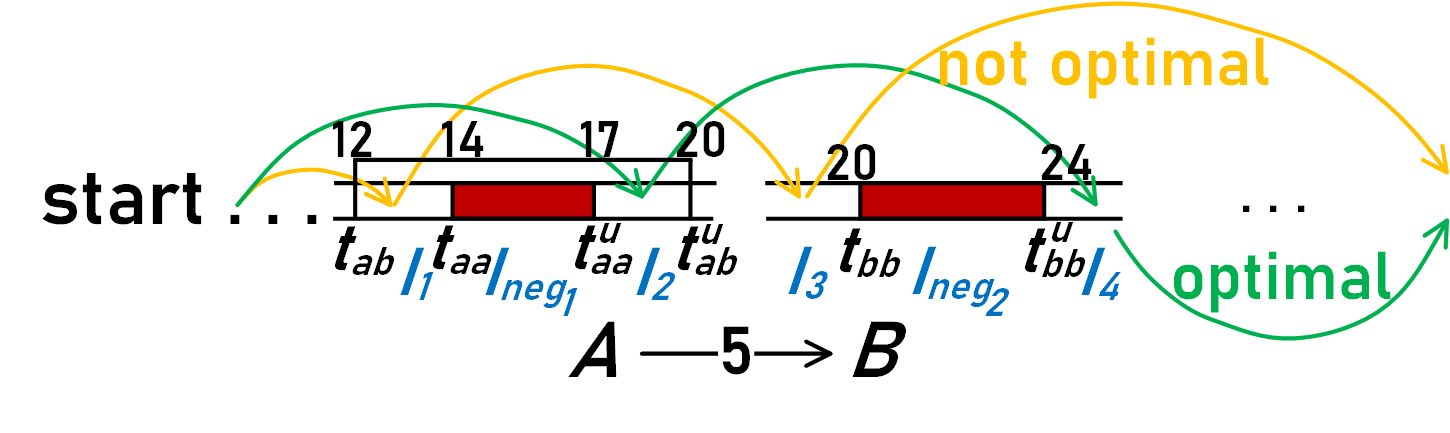
\includegraphics[width=0.9\columnwidth]{Example_diff_starts.png}
    \caption{An example where performing the action landmark as early as possible leads to a suboptimal plan.}
    \label{fig:early_plan_not_optimal}
\end{figure}
\begin{figure}
    \centering
    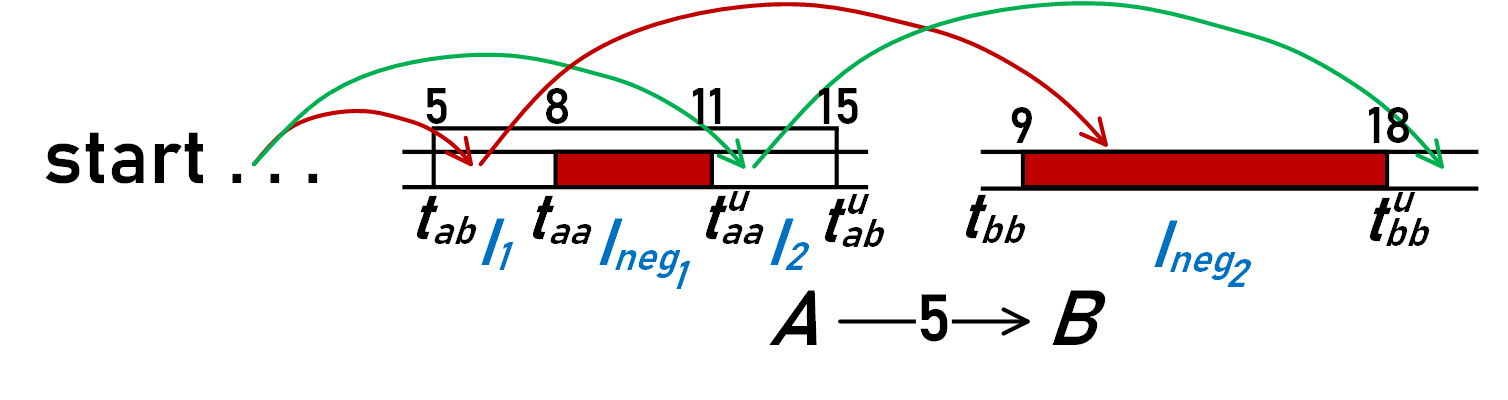
\includegraphics[width=0.9\columnwidth]{Example_diff_goals.png}
    \caption{An example where performing the action landmark as early as possible results in failing to find a plan.}
    \label{fig:early_plan_not_complete}
\end{figure}
% Example where earliest is not optimal 
Consider the illustration depicted in Figure~\ref{fig:early_plan_not_optimal}. 
The low-level search needs to find a plan that satisfies three constraints: 
\begin{itemize}
    \item A positive constraint $(i, \text{move(A,B)}, [t_{ab}, t_{ab}^u)$. 
    \item A negative constraint $(i, \text{wait\_at}(A), [t_{aa}, t_{aa}^u)$.
    \item A negative constraint $(i, \text{wait\_at}(B), [t_{bb}, t_{bb}^u)$.
\end{itemize}
where $t_{ab} < t_{aa} < t_{aa}^u < t_{ab}^u <t_{bb} < t_{bb}^u$. 
Thus, the negative constraint on waiting at $A$ ($\text{wait\_at}(A)$) creates two safe intervals for $A$,  $I_1=[0,t_{aa}]$ and $I_2=[t_{aa}^u,\infty)$, 
and the negative constraint on waiting at $B$ ($\text{wait\_at}(B)$) creates two safe intervals for $B$,  
$I_3=[0,t_{bb}]$ and $I_4=[t_{bb}^u,\infty)$. 
%corresponding to arriving at $A$ either before $t_{aa}$ or after $t_{aa}^u$. 


Now assume that there are two plans that satisfy the action landmark for the positive constraint, one that reaches $A$ before $t_{aa}$ (shown in yellow) and one that reaches $A$ after $t_{aa}^u$ (show in green). 
Clearly, the lowest-cost plan to achieve the action landmark is the one that reaches $A$ before $t_{aa}$, but to find the optimal solution one must use the second plan. 
Figure~\ref{fig:early_plan_not_complete} illustrates an even more extreme case, where choosing to lowest-cost plan that achieves the action landmark can not be extended to a full plan, because it reaches $B$ during its unsafe interval (marked in red). 

% \begin{observation}
% Finding the lowest-cost plan to achieve each action landmark is not sufficient to construct a plan that satisfies all given \ccbs constraints. 
% \end{observation}

% Assume now that $t_{ab} < t_{aa} < t_{aa}^u < t_{ab}^u$ (as shown on Fig.~\ref{fig:intervals_example}), which means that the negative constraint on waiting at $A$ splits the interval of the positive one. How the intermediate goal associated with the landmark $A \rightarrow B$ should like in this case? One option is $(A, I_1=[0, t_{aa}))$, another one is $(A, I_2 = [t_{aa}^u, t_{ab}^u))$, corresponding to the agent arriving to $A$ before the beginning of the unsafe waiting interval or after it. Actually, it is mandatory to simultaneously consider both goals.

% Here, the optimal solution 
% It may very well be that the optimal solution is 
% Now, assume that 
% The low-level search decomposes its task to (1) find a plan from $s(i)$ hat\emph{reach A at $[t_{ab}, t_{ab}^u)$}, 
% (2) perform the action landmark ($\text{move(A,B)}$), 
% and (3) \emph{reach the goal from $B$}. 


% However, there may be multiple plans that reach $A$ in the specified time range. 
% % In particular, when $t_{ab} < t_{aa} < t_{aa}^u < t_{ab}^u$ the negative constraint on waiting at $A$ creates two safe intervals for vertex $A$, corresponding to arriving at $A$ either before $t_{aa}$ or after $t_{aa}^u$. 
% Now assume that there are two plans that satisfy the action landmark for the positive constraint $(i, \text{move(A,B)}, [t_{ab}, t_{ab}^u)$, one that reaches $A$ before $t_{aa}$ and one after $t_{aa}^u$. 
% One may be tempted to choose the lowest cost plan to achieve this landmark, i.e., the plan that reaches $A$ sooner (=before $t_{aa}$). 

% Howeve,r , the lowest 
% As this example demonstrates, it is not sufficient to search for the lowest cost plan that satisfy this action landmark. 

% . 

% Informally, an agent has to find its individual plan that mandatory includes moving from $A$ to $B$ at some moment of the interval $I_{pos}$ and excludes waiting at $A$ within $I_{neg_1}$ and excludes arriving to  $B$ within $I_{neg_2}$. 

% Assume now that $t_{ab} < t_{aa} < t_{aa}^u < t_{ab}^u$ (as shown on Fig.~\ref{fig:intervals_example}), which means that the negative constraint on waiting at $A$ splits the interval of the positive one. How the intermediate goal associated with the landmark $A \rightarrow B$ should like in this case? One option is $(A, I_1=[0, t_{aa}))$, another one is $(A, I_2 = [t_{aa}^u, t_{ab}^u))$, corresponding to the agent arriving to $A$ before the beginning of the unsafe waiting interval or after it. Actually, it is mandatory to simultaneously consider both goals.

% The reason is that the interval of the negative constraint imposed over arriving/waiting at the target vertex of the landmark, $I_{neg_2}$, might eventually interfere with $I_1$ but not with $I_2$ (or vice versa), i.e. if an agent starts moving from $A$ to $B$ at any time moment from $I_1$ it always reaches $B$ at the unsafe interval $I_{neg_2}$, while reaching $B$ safely is possible from $I_2$ -- see Fig.~\ref{fig:intervals_example}.

% Moreover, even if $B$ is reachable from both $I_1$ and $I_2$ but the arrival times belong to different safe intervals of $B$, then, again, two transition options of going from $A$ to $B$ should be considered, as by considering only one option we might find non-optimal path from $B$ to the next landmark and therefore to the overall goal -- see Fig.~\ref{fig:different_starts_example}. This implies that in this case two distinct start nodes associated with $B$ must be introduced and incorporated into the search.


% Our solution 

% Pseudo code


% Positive constraints are handled as \emph{action landmarks}, i.e., actions that must be performed in any plan.\roni{Maybe cite some planning work on action landmarks} 
% Planning with action landmarks in our context can be done efficiently, as follows. 
% Similar to the low-level search in \cbsds, we sort the positive constraints in ascending order of their time dimension. 
% Then, sequentially plan from one landmark to the other, and the concatenation of these plans is the sought solution.


% Individual planning with landmarks in \ccbsds requires  careful reasoning about time intervals, especially, when both positive and negative constraints are simultaneously associated with them. In such cases multiple start/goal states for the individual planning might be introduced and considered -- a distinctive feature of low-level planning in \ccbsds not present in \cbsds.
% \roni{In my view this is where things gets interesting, but there is not enough details. How is this ``careful reasoning about time intervals'' being done? Maybe even a psuedo code. }\konstantin{Well, now it's illustrated via an example (with pictures). I agree that adding code might be beneficial. The thing is that the 'careful reasoning' applies only to the process of creating start/goal nodes associated with the landmarks. As for planning with multiple start/goals -- it is pretty straightforward (so, I think, no code is needed here as the difference from regular \sipp's code is negligible).}
%We, first, explain how planing is performed in case no negative constraints are present and then show how the introduction of such constraints may lead to planning with multiple start/goal states (a distinctive feature of low-level planning in \ccbsds).

%KONSTANTIN: Below was the text which is placed now in 'trimming-intervals.tex'. I don't think we need it now.




% \paragraph{Mutual effect of positive and negative time-interval constraints}

% \begin{figure}
%     \centering
%     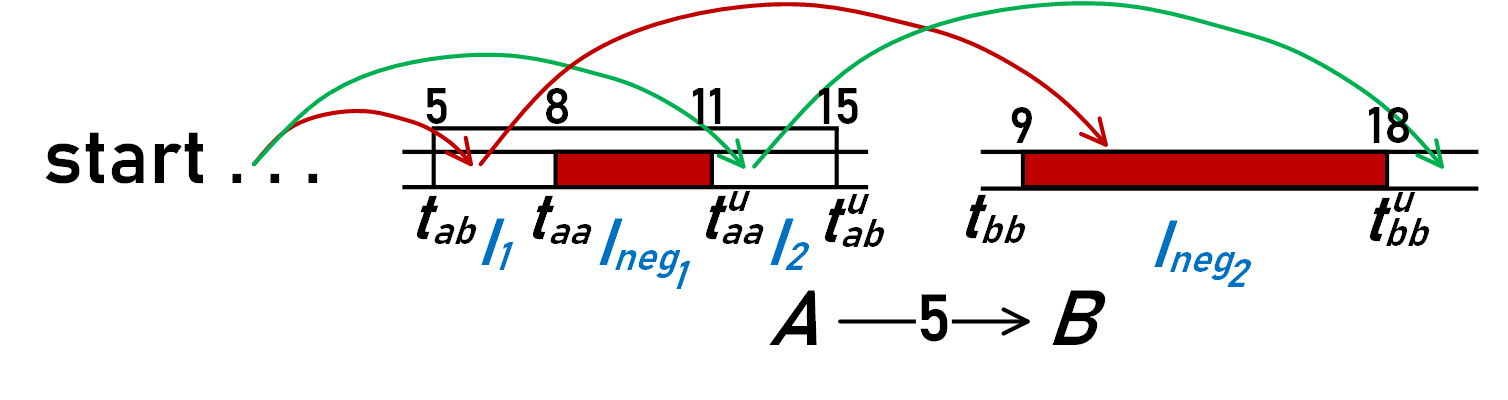
\includegraphics[width=\columnwidth]{Example_diff_goals.png}
%     \caption{Caption}
%     \label{fig:intervals_example}
% \end{figure}

% Consider an example, depicted on Fig.~\ref{fig:intervals_example}. Here an agent needs to find a plan that satisfies three constraints: 
% \begin{itemize}
%     \item A positive constraint associated with the move action $A \rightarrow B$ and the interval $I_{pos}=[t_{ab}, t_{ab}^u)$ (thus $A \rightarrow B$ is a landmark);
%     \item a negative constraint that prohibits waiting at $A$ at the time interval $I_{neg_1}=[t_{aa}, t_{aa}^u)$;
%     \item a negative constraint that prohibits waiting at $B$ at the time interval $I_{neg_2}=[t_{bb}, t_{bb}^u)$.
% \end{itemize}

% Informally, an agent has to find its individual plan that mandatory includes moving from $A$ to $B$ at some moment of the interval $I_{pos}$ and excludes waiting at $A$ within $I_{neg_1}$ and excludes arriving to  $B$ within $I_{neg_2}$. 

% Assume now that $t_{ab} < t_{aa} < t_{aa}^u < t_{ab}^u$ (as shown on Fig.~\ref{fig:intervals_example}), which means that the negative constraint on waiting at $A$ splits the interval of the positive one. How the intermediate goal associated with the landmark $A \rightarrow B$ should like in this case? One option is $(A, I_1=[0, t_{aa}))$, another one is $(A, I_2 = [t_{aa}^u, t_{ab}^u))$, corresponding to the agent arriving to $A$ before the beginning of the unsafe waiting interval or after it. Actually, it is mandatory to simultaneously consider both goals.

% The reason is that the interval of the negative constraint imposed over arriving/waiting at the target vertex of the landmark, $I_{neg_2}$, might eventually interfere with $I_1$ but not with $I_2$ (or vice versa), i.e. if an agent starts moving from $A$ to $B$ at any time moment from $I_1$ it always reaches $B$ at the unsafe interval $I_{neg_2}$, while reaching $B$ safely is possible from $I_2$ -- see Fig.~\ref{fig:intervals_example}.

% Moreover, even if $B$ is reachable from both $I_1$ and $I_2$ but the arrival times belong to different safe intervals of $B$, then, again, two transition options of going from $A$ to $B$ should be considered, as by considering only one option we might find non-optimal path from $B$ to the next landmark and therefore to the overall goal -- see Fig.~\ref{fig:different_starts_example}. This implies that in this case two distinct start nodes associated with $B$ must be introduced and incorporated into the search.

\subsubsection{Generalized \sipp}

% Key: find best plan per safe interval
 
 There may be an infinite plans that satisfy a given action landmark $l=(i, \text{move}(A,B), [t,t^u))$ and it is not sufficient to only find the lowest-cost one. 
 However, it is sufficient to find the lowest-cost plan to reach $A$ \emph{for every safe interval} of $A$ that overlaps with $[t,t^u)$.  
%   Based on this observation we propose the following low-level search for \ccbsds. 
 % Consider a landmark $l=(i, \text{move}(A,B), [t,t^u))$ and a set of negative constraints $C_1, ..., C_k$ imposed on waiting at $A$ with the intervals $I_{neg_1}= [t_1, t_1^u)$, ..., $I_{neg_k}=[t_k, t_k^u)$, s.t. $I_{neg_1} \cap [t,t^u) \neq \emptyset$, ...,  $I_{neg_k} \cap [t,t^u) \neq \emptyset$ and $t_1 > t$ and $t_k^u < t^u$\footnote{The corner cases when $t_1 > t$ or $t_k^u < t^u$ are treated similarly.}.  Then the following \sipp goal nodes are defined for planning to $l$ from the preceding landmark: $goal_1=(from(a), [t, t_1))$, $goal_2=(from(a), [t_1^u, t_2))$, ..., $goal_k=(from(a), [t_{k-1}^u, t_k])$, $goal_{k+1}=(from(a), [t_k^u, t^u))$. 
%  , and construct an overall plan wi
% %  That is, the optimal plan that satisfies all the given \ccbs constraints 
%  can be decomposed into sub-plans that achieve the action landmarks one after the other
 
 
 To this end, we create a generalized version of \sipp such that: 
 (1)  it accepts a set of goal states, one per safe interval of $A$ that overlaps with $[t,t^u)$, 
 and (2) it outputs a set  plans, one per goal state. 
 To each of these plans, we concatenate the  action landmark itself $\text{move}(A,B)$. 
 These plans may end in different safe intervals in $B$, which will then be distinct start states when searching for a plan to get from $B$ to the next landmark. 
Thus, our generalized \sipp accepts a set of starts states and a set of goal states and outputs a set of plans, one per goal. 
It works as follows. 
First, the open list (denoted \open) is initialized with 
\emph{all} start states. 
Then, the search proceeds as in regular \sipp, except that the the stop criteria is either when \open is exhausted or when \emph{all} goal nodes are expanded. 

% such that every returned plan is a lowest cost plan to one of the goals sfrom one of the start states.  
%  , 
%  (3) it accepts a set of start states. 
%  The latter is needed because the returned plans form the start states for finding the plan to reach the next action landmark. 
%  The 



\subsubsection{Pseudo Code}

%version described above, which initiated OPEN with the set of nodes in \emph{starts} and halts when it expands all nodes in \emph{goals}. 

\begin{algorithm}
    \KwIn{Negative constraints $C^{(-)}$}
    \KwIn{Positive constraints $C^{(+)}$}
    \KwIn{Agent $i$}
    %   \KwOut{bla}
    Starts $\gets \{(s_i,0)\}$\\
    $\cal S\gets$ ComputeSafeIntervals($C^{(-)}$)\\
    $\cal L \gets$ ComputeLandmarks($C^{(+)}$, $g_i$, $\cal S$)\\
        \ForEach{landmark $l=(i,\text{move}(A,B),[t,t^u))$ in $\cal L$}{
                Goals $\gets$ computeGoals(l)\\
                plans $\gets$ \sipp(Starts, Goals)\\
                Starts $\gets \emptyset$\\
                \ForEach{plan in Plans}{
                    Append $a$ to $plan$\\
                    Merge plans if possible
                    % (plan[-1])$ to Starts 
                    % %reached by performing action $a$ at the end of plan 
                }
            }
		\Return the first plan in plans
	\caption{Low-level search for \ccbs with \ds} 
\label{alg:low-level-ccbs-ds}
\end{algorithm}

Finally, we can describe the pseudo-code for the \ccbsds low-level search. It accepts a list of negative and positive constraints for an agent $i$. Let \sipp(Starts, Goals) denote our generalized \sipp. 
Initially, the low-level search computes the safe intervals of every vertex based on the negative constraints. 
Then, it computes the action landmarks based on the positive constraints. 
These landmarks are sorted by time, and then it iterates over these landmarks. 
For each action landmark $l=(i,\text{move}(A,B),[t,t^u))$, it computes the safe intervals of $A$ that intersect with $[t,t^u)$. 
Every such safe interval is considered a goal for our generalized \sipp. 
When all such goals are added, we run our generalized \sipp to find a set of plans, one per goal. Then, we concatenate to the end of each of these plans the action $\text{move}(A,B)$, 
and compute from this the set of start states for the next iteration. 

% Thus, the low-level search in \ccbsds is a generalization of \sipp that accepts a set of start states and a set of goal states and returns the lowest cost plan to every goal state. 
% This generalized \sipp works as follows. 
% First, the open list (denoted \textit{OPEN}) is initialized with 
% \emph{all} start states. 
% Then, the search proceeds as in regular \sipp, except that the the stop criteria is either when \textit{OPEN} is exhausted or when \emph{all} goal nodes are expanded. 

% \textbf{Defining the goal nodes} Consider a landmark $l=(i, a, [t,t^u))$ and a set of negative constraints $C_1, ..., C_k$ imposed on waiting at the vertex $from(a)$ with the intervals $I_{neg_1}= [t_1, t_1^u)$, ..., $I_{neg_k}=[t_k, t_k^u)$, s.t. $I_{neg_1} \cap [t,t^u) \neq \emptyset$, ...,  $I_{neg_k} \cap [t,t^u) \neq \emptyset$ and $t_1 > t$ and $t_k^u < t^u$\footnote{The corner cases when $t_1 > t$ or $t_k^u < t^u$ are treated similarly.}.  Then the following \sipp goal nodes are defined for planning to $l$ from the preceding landmark: $goal_1=(from(a), [t, t_1))$, $goal_2=(from(a), [t_1^u, t_2))$, ..., $goal_k=(from(a), [t_{k-1}^u, t_k])$, $goal_{k+1}=(from(a), [t_k^u, t^u))$. 

% \textbf{Defining the start nodes} Start nodes are defined similarly to the goal ones with the substitution of $from(a)$ to $to(a)$. 


Note that the number of returned plans in every call to our generalized \sipp is always limited by the number of start nodes of the subsequent landmark and the latter is proportional to the number of the negative constraints associated with the wait actions 
for the source vertex of the landmark (as explained above). 
Consequently, if no wait actions are prohibited at the vertex which is the source of the landmark then only one plan to this landmark is built (no matter with how many different start nodes the search was initialized). 
That means that in the process of the iterative invocation of the modified \sipp numerous plans constructed so far might eventually collapse to a single one. This definitely happens when one is planning to the final goal. The reason is that this goal is defined by a single graph vertex and a single time interval ending with $\infty$ (recall that we assume that the agent arrives to its goal and stays there forever). Thus, even if numerous plans to the preceding landmark were found they all will collapse into a single one, i.e. the one that achieves the final goal at the earliest possible time (the plans that achieve this goal later are discarded).
 
 
 
 
 
 
 
% The \ccbsds low-level search 
% From the examples above, we observed that in t

% in \ccbsds is that there may be an infinite plans that satisfy a given action landmark $l=(i, \text{move}(A,B), [t,t^u))$ and it is not sufficient to only find the lowest-cost one. 

% it is sufficient to return a single lowest-cost plans that reaches $A$ 
% \emph{for each} safe interval of $A$ in the range $[t,t$

% except  
% to find an optimal plan it is sufficient to only find the lowest-cost plan to an action land mark \emph{for every safe interval}. 

% that satisfies a given set of \ccbs constraints it is sufficient to find 

% while it is not sufficient to find only the lowest-

% In general numerous start/goal nodes can be defined for the individual planner due to the existence of the negative constraints associated with the landmarks' endpoints (i.e. the vertices defining the landmarks). The number of that nodes is finite and is proportional to the number of the negative constraints imposed on the wait actions associated with the vertices defining that landmarks. Next we present formal ways to define start and goal nodes.







%As a result, the overall plan from the agent's start to the agent's goal containing the mandatory $A \rightarrow B$ action will not be found if only option of reaching $A$ within $I_1$ is considered. To account for this we split the \sipp node $(A, I_{neg})$ into the $(A, I_1)$, $(A, I_2)$ and treat them as separate sub-goals during the search.


%Finding the plans to the separate goal nodes, $goal_1=(v, [t,t'])$, $goal_2=(u, [t'', t'''])$ (no matter whether $v$ and $u$ are the same vertex or the separate ones) with \sipp can be implemented by keeping the algorithm's structure the same but modifying the stop criterion as follows. The search should be stopped if either of the following occurs:
%\begin{itemize}
%    \item \emph{OPEN} is exhausted;
%    \item $goal_1$ is retrieved from \emph{OPEN} to be expanded \texttt{and} $goal_2$ has already been expanded;
%    \item $goal_2$ is retrieved from \emph{OPEN} to be expanded \texttt{and} $goal_1$ has already been expanded;
%\end{itemize}

%In the last two cases, according to SIPP's properties, one can infer that the optimal plans to $goal_1$ and $goal_2$ have been found and can be reconstructed using the pointers to the predecessors in the search tree. Indeed, it is assumed that the heuristic function that guides the search is consistent.

%Moreover one can add to the stop criterion the following condition in order to possibly reduce the search effort: if the $f$-value of the node under expansion exceeds $max(t'+h(goal_1), t'''+h(goal_2))$ the search must halt. Obviously, if by that iteration $goal_1$ (or $goal_2$) was not expanded so far (and $h$ is consistent) one won't reach it in the appropriate time interval further on. 


%A straightforward way to incorporate this to \sipp is to define a search node $x=(A, [t_{ab}, t_{ab}^u))$ and adjust the search as follows:
%\begin{itemize}
%    \item Find a plan from the start vertex to node $x$. This plan either does not exist (in this case the search reports \emph{failure} and the proccess is halted) or it exists and ends with arriving at $A$ at some time moment $t^* \in [t_{ab}, t_{ab}^u)$.
%    \item Perform move action $A \rightarrow B$ at the earliest possible moment belonging to the interval $[t^*, t_{ab}^u)$, s.t. the arrival time does not violate with any of the \ccbs constraints assosiated with arriving/waiting at $B$. In case such move can not be performed halt the search.
%    \item Start a fresh \sipp search from the node $(B, [begin(interval(t^*)), end(interval(t^*))])$ to the goal node. Here $begin(interval(t))$ and $end(interval(t))$ denote the time moment that define an interval to which $t$ belongs.
%\end{itemize}


%In case of \ccbs which uses \sipp this is not straightforward as requires careful reasoning about two kinds of time intervals: intervals which are part of the negative constraints and intervals that are part of the positive constraints.

%Consider an example, depicted on Fig.~\ref{fig:intervals_example}. Assume that an agent has a positive constraint associated with the move action $A \rightarrow B$ and an interval $[t_{ab}, t_{ab}^u)$. Moreover, assume that there is a negative constraint over the wait action $B \rightarrow B$ at time interval $[t_{bb}, t_{bb}^u)$. That is, an agent is not allowed to come to (and/or wait at) $B$ in that interval. Suppose now that $t_{ab} + d(A \rightarrow B) < t_{bb} < t_{bb}^u < t_{ab}^u + d(A \rightarrow B)$, where $d(A \rightarrow B)$ is the duration (cost) of the corresponding move action. In that situation in order to find a safe path for an agent to its goal the planner should consider two alternative possibilities to arrive at $B$, both consistent with the current positive and negative constraints. One option is to reach $B$ at $[t_{ab} + d(A \rightarrow B), t_{bb}]$. Another one is to reach $B$ at $[t_{bb}^u, t_{ab}^u + d(A \rightarrow B)]$. Both options should be considered as in case one of the intervals is discarded a path to a goal may not be found despite it exists and is reachable trough the \sipp search node containing the discarded interval.






% \subsection{Theoretical properties}
% Need to show that CCBS with disjoint splitting is correct, sound, complete, optimal.
% \konstantin{Do we need this? Original paper on \cbsds did not contain any theoretical claims/proofs. If we opt to have it here - we need a proof (I did not think about it and I'm not sure that will have time to.}
% \roni{Let's comment this out for now, and I'll try to create a nice proof that we can either add here or have as supplamentary material and have here just the Theorem}





% \subsection{Enhancements for CBS}
% A range of significant improvements for \cbs have been introduced that greatly improve its computational efficiency~\cite{}. % of the algorithm, and in particular its ability to find optimal solutions to complex \mapf problems in limited time. 
% Among them are: \pc~\cite{boyarski2015icbs}, adding heuristics to high-level search~\cite{}, \ds~\cite{}, reasoning over symmetries~\cite{} etc. Further we give a brief overview of the techniques that are relevant to this work.



\section{Prioritizing Conflicts}

%Reminder: what is PC in classical CBS

%Observation: in CCBS almost all conflicts are cardinal

%Our approach: prioritize by min. cost increase of the pair

%For every CCBS conflict $Con=(i,j,a_i,a_j)$ 
%let $\Delta Con=(\delta_i, \delta_j)$ where $\delta_i$ is the increase in cost for agent $a_i$ if it is replanning with the additional constraint to avoid the conflict $Con$. 
%We currently choose the conflict $Con$ that maximizes $\min(\Delta Con)$. I'll call this prioritize by min. cost increase. Alternatively, we could choose the conflict that maximizes $\max(\Delta Con)$. I'll call this prioritize by max. cost increase.

%(Maybe do some minimal experiments checking sum, average, max)

%We can compare:
%1) Prioritize by time (max or min, whichever works best) 
%2) Prioritize by min. cost increase
%3) Prioritize by max. cost increase

\acf{PC} is the second \cbs enhancement we migrate to \ccbs. 
\pc is a heuristic for choosing which conflict to resolve when expanding a \ct node. 
Such a heuristic is needed when the \cbs high-level search expands a node $N$ having multiple conflicts in its joint plan ($N.\Pi$). % is used
% when processing a \ct-node, \cbs arbitrarily chooses a conflict to resolve. 
Different ways to choose conflicts in practice often lead to \ct of different sizes, 
thus have a significant effect on the overall runtime. 
\pc systematically prioritizes conflicts by classifying each conflict as either \emph{cardinal}, \emph{semi-cardinal}, and \emph{non-cardinal}. 
A conflict $(i,x,t)$ is called cardinal \emph{iff} splitting a \ct node $N$ over it results in two child nodes
whose cost is higher than the cost of $N$. 
A conflict is semi-cardinal \emph{iff} if the cost of only one child increases while the cost of the other does not. 
A conflict that is not cardinal or semi-cardinal is non-cardinal. 
%, non-cardinal in all other cases. For splitting a node \icbs prefers cardinal conflicts to semi-cardinal and semi-cardinal to non-cardinal. 
\cbs with \pc prefers cardinal conflicts to semi-cardinal and semi-cardinal to non-cardinal.  
%to expand  
This way of prioritizing conflicts results in a significant reduction of the expanded \ct nodes compared to vanilla \cbs and makes the algorithm much faster in practice.


% \pc for \cbs won't work for \ccbs
In \mapfr, most conflict are cardinal, i.e. the agents involved in that conflict are not able to find the paths that respect the corresponding constraints and are of the same cost as before. The reason for that is that the ability to perform wait actions of arbitrary duration paired with non-uniform costs of the move actions reduces the symmetry in \mapfr setting. 
Thus, differentiating the conflicts based just on their cardinality type is insufficient.


To this end, we propose a generalized version of \pc that introduces a finer-grained prioritization of conflicts, by introducing the notion of \emph{cost impact}. 
Intuitively, the cost impact of a conflict is how much the cost of the solution is increased when it is resolved. %a cardinal conflict is resolved. 
\roni{Eli, if you happen to have time, take a look at this and see if I'm missing something regarding your very latest work on f-cardinal conflicts and all that}\eli{looks fine}
More formally, for a \ct node $N$ with a \ccbs conflict $Con=(a_i, t_i, a_j, t_j)$, 
let $N_i$ and $N_j$ be the \ccbs nodes obtained by splitting over this conflict, 
and let $\delta_i$ be the difference between the cost of $N$ and $N_i$. 
We define the \emph{cost impact} of the conflict $Con$, denoted $\Delta(Con)$, as $\min(\delta_i, \delta_j)$.
\footnote{We also experimented with $\Delta(Con) = \max(\delta_i, \delta_j)$ and $\Delta(Con) = \sum(\delta_i, \delta_j)$ but it resulted in only  slight shifts in the performance.}
Our adaptation of \pc to \ccbs chooses to split a \ct node on the conflict with the largest cost impact. 
\roni{Maybe add a line on how this captures the same rationale as \pc for \cbs.}

% The conflict with the lowest cost impact is chosen by \ccbs when using \pc. 

% : (\delta_i, \delta_j) \rightarrow [0; +\infty)$. E.g. $\Delta(Con)$ can be defined as $min(\delta_i, \delta_j)$, $max(\delta_i, \delta_j)$, $sum(\delta_i, \delta_j)$ etc. 

% When $\Delta(Con)$ is defined the cardinal and semi-cardinal conflicts can, indeed, be prioritized based on their $\Delta$-value. In our experiments we set $\Delta Con$ to be $min(\delta_i, \delta_j)$ and prefer conflicts with larger values of $\Delta$. We also experimented with $\Delta(Con) = max(\delta_i, \delta_j)$ and $\Delta(Con) = sum(\delta_i, \delta_j)$ but evidenced only slight shifts in the performance of the algorithm.


%\pc~\cite{boyarski2015icbs} is a powerful technique for \cbs that aims at reducing the number of \ct nodes expansions by introducing a partial order on the set of conflicts associated with every \ct node. I.e. all conflicts are partitioned to three priority classes: \emph{cardinal}, \emph{semi-cardinal} and \emph{non-cardinal} based on how the cost of the solution increases when a conflict is eliminated. If elimination of a conflict leads to increasing the costs of the individual solutions of both agents involved in a conflict, the latter is classified as cardinal, if the cost increases for only one agent but not for the other, the conflict is classified as semi-cardinal. In all other cases the conflict is non-cardinal. Now, \cbs prefers to split each \ct by first choosing cardinal conflicts, then semi-cardinal and then non-cardinal.

%Prioritizing Conflicts enhancement for classical CBS was introduced in [ICBS]. There were introduced three types of conflicts: cardinal, semi-cardinal and non-cardinal. Conflict $Con=(i,j,a_i,a_j)$ is cardinal if its elimination is impossible without increasing in the solution cost. In other words, both of the replanned trajectories for agents $i$ and $j$ that satisfy the corresponding  constraints $C_1=(i, a_i, [t_i, t_i^u))$, $C_2=(j, a_j, [t_j, t_j^u))$ have increased costs. If only one of the replanned trajectories has an increased cost, then conflict $Con$ is semi-cardinal. Otherwise, its non-cardinal.

%To guarantee optimality, CBS expands CT-nodes in the best-first order according to their costs, i.e. always chooses the one with minimal cost. The cost of the child nodes depends on the type of conflict that was chosen for split. Preferring to split the cardinal conflicts before semi-cardinal or non-cardinal conflicts and semi-cardinal before non-cardinal conflicts, the one can increase the cost of child nodes and further to increase the minimal cost in CT-tree. Thus to get closer to the collision-free solution and to spend less expansions. 

%To detect cardinal and semi-cardinal conflicts, the authors of ICBS[] suggested to use multi-value decision diagrams (MDD)[]. Each $MDD^c_i$ contains all possible paths of a predefined cost $c$ for some agent $i$. Nodes of the MDD can be distinguished by their depth below the source node. Every node at depth $t$
%of $MDD^c_i$ corresponds to a possible location of agent $i$ at time $t$. In cases when the constraint is imposed on some location at time $t$ which is the only option at the depth $t$, it definitely leads to an increase of the trajectory cost.

%Detection of the types of conflicts and resolving them in a proper order allowed sped up classical CBS and reduced the number of expanded CT-nodes up to one order of magnitude in the tested scenarios \cite{ICBS}.

%This enhancement can be applied to CCBS as well. However, it has the following peculiar properties:

%1) Use of MMDs for detection of cardinal and semi-cardinal conflicts is impossible, due to the presence of continuous time and actions of non-uniform cost. I.e. there are no time-steps, depth-levels, etc. The only way is to replan the agent's trajectory with respect to the corresponding constraint and compare the costs.

%2) The cost increases from resolving cardinal conflicts in CCBS can vary. They depend on the cost increases that both agents incur, i.e. $\Delta Con=(\delta_i, \delta_j)$ where $\delta_i$ is the increase in cost for agent $i$ if it is replanned with the additional constraint to avoid the conflict $Con$. As a singular cost increase value, $\Delta Con$ could be defined in a few ways, such as $min(\delta_i, \delta_j)$, $max(\delta_i, \delta_j)$, or $sum(\delta_i, \delta_j)$. However, our preliminary tests have shown that there is almost no difference between these options, at least in terms of the amount of successfully solved instances.

%3) This property follows in a consequence of the previous point. In case of presence of several cardinal conflicts, they can be compared and prioritized as well. Obviously, the most promising way is to choose the conflict with maximum cost increase as it helps to increase the solution cost the most.

\section{Heuristics for High-Level Search}



% \paragraph{Adding heuristics to high-level search.} \Roni{maybe this is a repetition}
% Originally \cbs explores the constraint tree in a best first manner picking a leaf $N$ with the lowest cost at each iteration. In~\cite{} an admissible heuristic that estimates by how much the cost of $N$ differs from the cost of an optimal \mapf solution was proposed. A resultant algorithm, \cbsh, explores the \ct tree in \astar fashion, i.e. on each iteration a \ct node $N$ is chosen to be processed that minimizes $g(N)+h(N)$, where $g(N)$ is the cost of the node and $h(N)$ is the introduced heuristic estimate. More involved and accurate heuristics were proposed in~\cite{}. \konstantin{Some quantative results saying how well introducing H affects CBS.}.

To guarantee optimality, the high-level search in \cbs explores the \ct tree in a best-first fashion, expanding in every iteration the \ct node in \open with the smallest cost. % (\soc) of the nodes' joint plan ($N.\Pi$). %sum-of-costs of the individual plans associated with the nodes. 
\citet{CBSH} and \citet{CBSH2} introduced admissible heuristics to the \cbs high-level search. 
These heuristics estimates the cost difference between the cost of a node and the cost of the optimal solution. Both heuristics are \emph{admissible}, i.e., they are a lower bound on the actual cost difference, and therefore can be safely added to the cost of a \ct node when choosing which node to expand next from \open. 
Improved heuristics were later suggested in~\cite{CBSH2}. 
Indeed, these heuristics were shown to significantly decrease the number of the expanded \ct nodes and improve the performance of \cbs. 


Drawing from these works we suggest two admissible heuristics for \ccbs. 
The first admissible heuristic, denoted $H1$, is based on solving the following linear programming problem (LPP). 
This LPP has $n$ non-negative variables $x_1,\ldots x_n$. 
Each conflict $Con_{i,j}$ between agents $i$ and $j$ 
in the \ct node for which we are computing the heuristic
introduces the LPP constraint $x_i + x_j \geq \Delta(Con_{i,j})$. 
The objective to be minimized is $\sum_{i=1}^n{x_i}$. 
By construction, for any solution to this LPP, the value $\sum_{i=1}^n{x_i}$ is an admissible heuristic since for every conflict $Con_{i,j}$ the solution cost is increased by $\Delta(Con_{i,j})$. 
\roni{Not an ideal proof, but, sufficient I think for a conference paper. I don't think it is hard to fully prove this in a formal way, but no time now.}

% Indeed, by following this approach one never overestimates the value by which the cost of a current \ct will increase in case all of its conflicts are resolved. Thus the resultant heuristic function is admissible. 


% For the \ct node for which we compute the $N$, let $x_i$ be the minimum cost increase that results from resolving \emph{all} conflicts in $N.\Pi$ that involve agent $i$.


% Consider the following 
% For a \ct node $N$, let $x_i$ be the minimum cost increase that results from resolving \emph{all} conflicts in $N.\Pi$ that involve agent $i$.
% By construction, the sum of the components $x_1$, $x_2$, ..., $x_n$ an admissible heuristic. 
% \roni{No this is incorrect. If $x_i$ was indeed what we write above, then the sum would not be admissible since maybe the minimum increase due to one agent also covers the minimum increase due to another agent.}
% To obtain a lower-bound estimate of all the $x_i$ components, one can solve the following linear programming problem (LPP). 
% Each conflict $Con$ between agents $i$ and $j$ introduces a LPP constraint: $x_i + x_j \geq \Delta(Con)$. 
% The objective to be minimized is $\sum_{i=1}^n{x_i}$. 
% Indeed, by following this approach one never overestimates the value by which the cost of a current \ct will increase in case all of its conflicts are resolved. Thus the resultant heuristic function is admissible. 



% Drawing from these works we suggest the following admissible heuristics for \ccbs. 
% For a \ct node $N$, let $x_i$ be the minimum cost increase that results from resolving \emph{all} conflicts in $N.\Pi$ that involve agent $i$.
% By construction, the sum of the components $x_1$, $x_2$, ..., $x_n$ an admissible heuristic. 
% \roni{No this is incorrect. If $x_i$ was indeed what we write above, then the sum would not be admissible since maybe the minimum increase due to one agent also covers the minimum increase due to another agent.}
% To obtain a lower-bound estimate of all the $x_i$ components, one can solve the following linear programming problem (LPP). 
% Each conflict $Con$ between agents $i$ and $j$ introduces a LPP constraint: $x_i + x_j \geq \Delta(Con)$. 
% The objective to be minimized is $\sum_{i=1}^n{x_i}$. 
% Indeed, by following this approach one never overestimates the value by which the cost of a current \ct will increase in case all of its conflicts are resolved. Thus the resultant heuristic function is admissible. 

% Let a heuristic be represented by the sum of the components $x_1$, $x_2$, ..., $x_n$, where $x_i$ is the minimum cost increase that results from \emph{all} conflicts involving agent $i$ are resolved. By the virtue of construction such a heuristic is an admissible one. To compute $x_i$ it is sufficient to solve the linear programming problem (LPP), which is defined as follows. Each conflict between agents $i$ and $j$ introduces a LPP constraint: $x_i + x_j \geq \Delta(Con)$, where $\Delta(Con)$ is computed as $min(\delta_i, \delta_j)$. The objective to be minimized is $\sum{x_i}$. Indeed, by following this approach one never overestimates the value by which the cost of a current \ct will increase in case all of its conflicts are resolved. Thus the resultant heuristic function is admissible. 


%function rely on detection of cardinal conflicts, and on their property that the resulting solution cost is increased by at least 1 relative to the parent node. This property is valid for classical \mapf where only uniform-cost actions are allowed. However, as mentioned before, resolving cardinal conflicts in \mapfr can lead to different cost increases, which can be greater than or lower than 1.

%Among the ways mentioned above that $\Delta(Con)$ values for cardinal conflicts $Con$ could be defined, the only one that guarantees the admissibility of the resulting h-value is defining it as $min(\delta_i, \delta_j)$, i.e. the cost increase of a cardinal conflict is equal to the minimum between the two increases in cost.

%One of the possible ways to calculate the high-level heuristic is to solve the linear programming problem (LPP). Each cardinal conflict is a constraint of the following form: $i_j + i_k \geq d_n$, where $i_j, i_k$ are the agents' indices between which the conflict occurs, $d_n$ - its cost increase. The number of LPP constraints is equal to the number of cardinal conflicts. The objective function of LPP is to minimize the total sum: $\sum{i_j}\rightarrow min$, where $j$ is the total amount of agents in the considered CT-node that have at least one cardinal conflict.

The second admissible heuristic we propose, denoted $H2$, follows the approach suggested in~\cite{CBSH}. 
There, the heuristic was based on identifying \emph{disjoint cardinal conflicts}, which are cardinal conflicts between disjoint pairs of agents. 
As discussed above, in \ccbs most conflicts are cardinal but their \emph{cost impact} can vary greatly. 
Therefore, in the $H2$ heuristic we aim to choose the disjoint cardinal conflicts that would have the largest cost impact. We do so in a greedy manner, sorting the conflicts in $N.\Pi$ in descending order of their cost impact. Then, conflicts are picked one by one in this order. 
After a conflict is picked, we remove from the conflict list all conflicts that involve at least one of the agents in this conflict. This process continues until all the conflicts are either picked or removed. 
The $H2$ heuristic is the sum of the cost impacts of the chosen conflicts. 
By construction the chosen conflicts are disjoint and so $H2$ is admissible. 
%Finally, $\Delta$ values of the picked conflicts are summed up to form a heuristic. 
While $H2$ is less informed than $H1$ (the one computed by solving LPP), it is faster to compute. 
We observed experimentally that the practical difference between these heuristics was negligible -- an average difference of 1\%. 
%--  both of them result in the very close values in almost all cases - the difference is less than 1\% in average. 
Thus, in for the experimental results below we used $H2$ and refer to it as $H$. 
%we used a second heuristic, i.e. the one that does not involve solving LPP.

%As well as in the original approach, we are looking for the disjoint cardinal conflicts, i.e. the conflicts between non-intersecting pairs of agents. The difference between them is that in CCBS cardinal conflicts have different cost increases associated with them and we can prioritize them using this information. We sort all the cardinal conflicts in the descending order. Further we just need to pick conflicts one by one, discarding all the conflicts that contain at least one of the agents from the already picked conflicts, until all the conflicts will be either picked or discarded. Summing the cost increases associated with all the picked conflicts we can get an admissible heuristic with values that can be equal or lower than the values obtained by the approach based on solving LPP. However, it can be calculated much faster as its complexity is pretty low.

%Our preliminary empirical evaluation has shown that both of the suggested approaches to calculate high-level heuristics provide almost equal h-values. The difference between the values is only about 1\% in average and they are totally equal in more than 94\% of cases (expanded CT-nodes). That is why in all the reported experimental results there is only one h-value - the one based on disjoint cardinal conflicts.

\section{Empirical Evaluation}

\begin{figure*}[t]
    \centering
    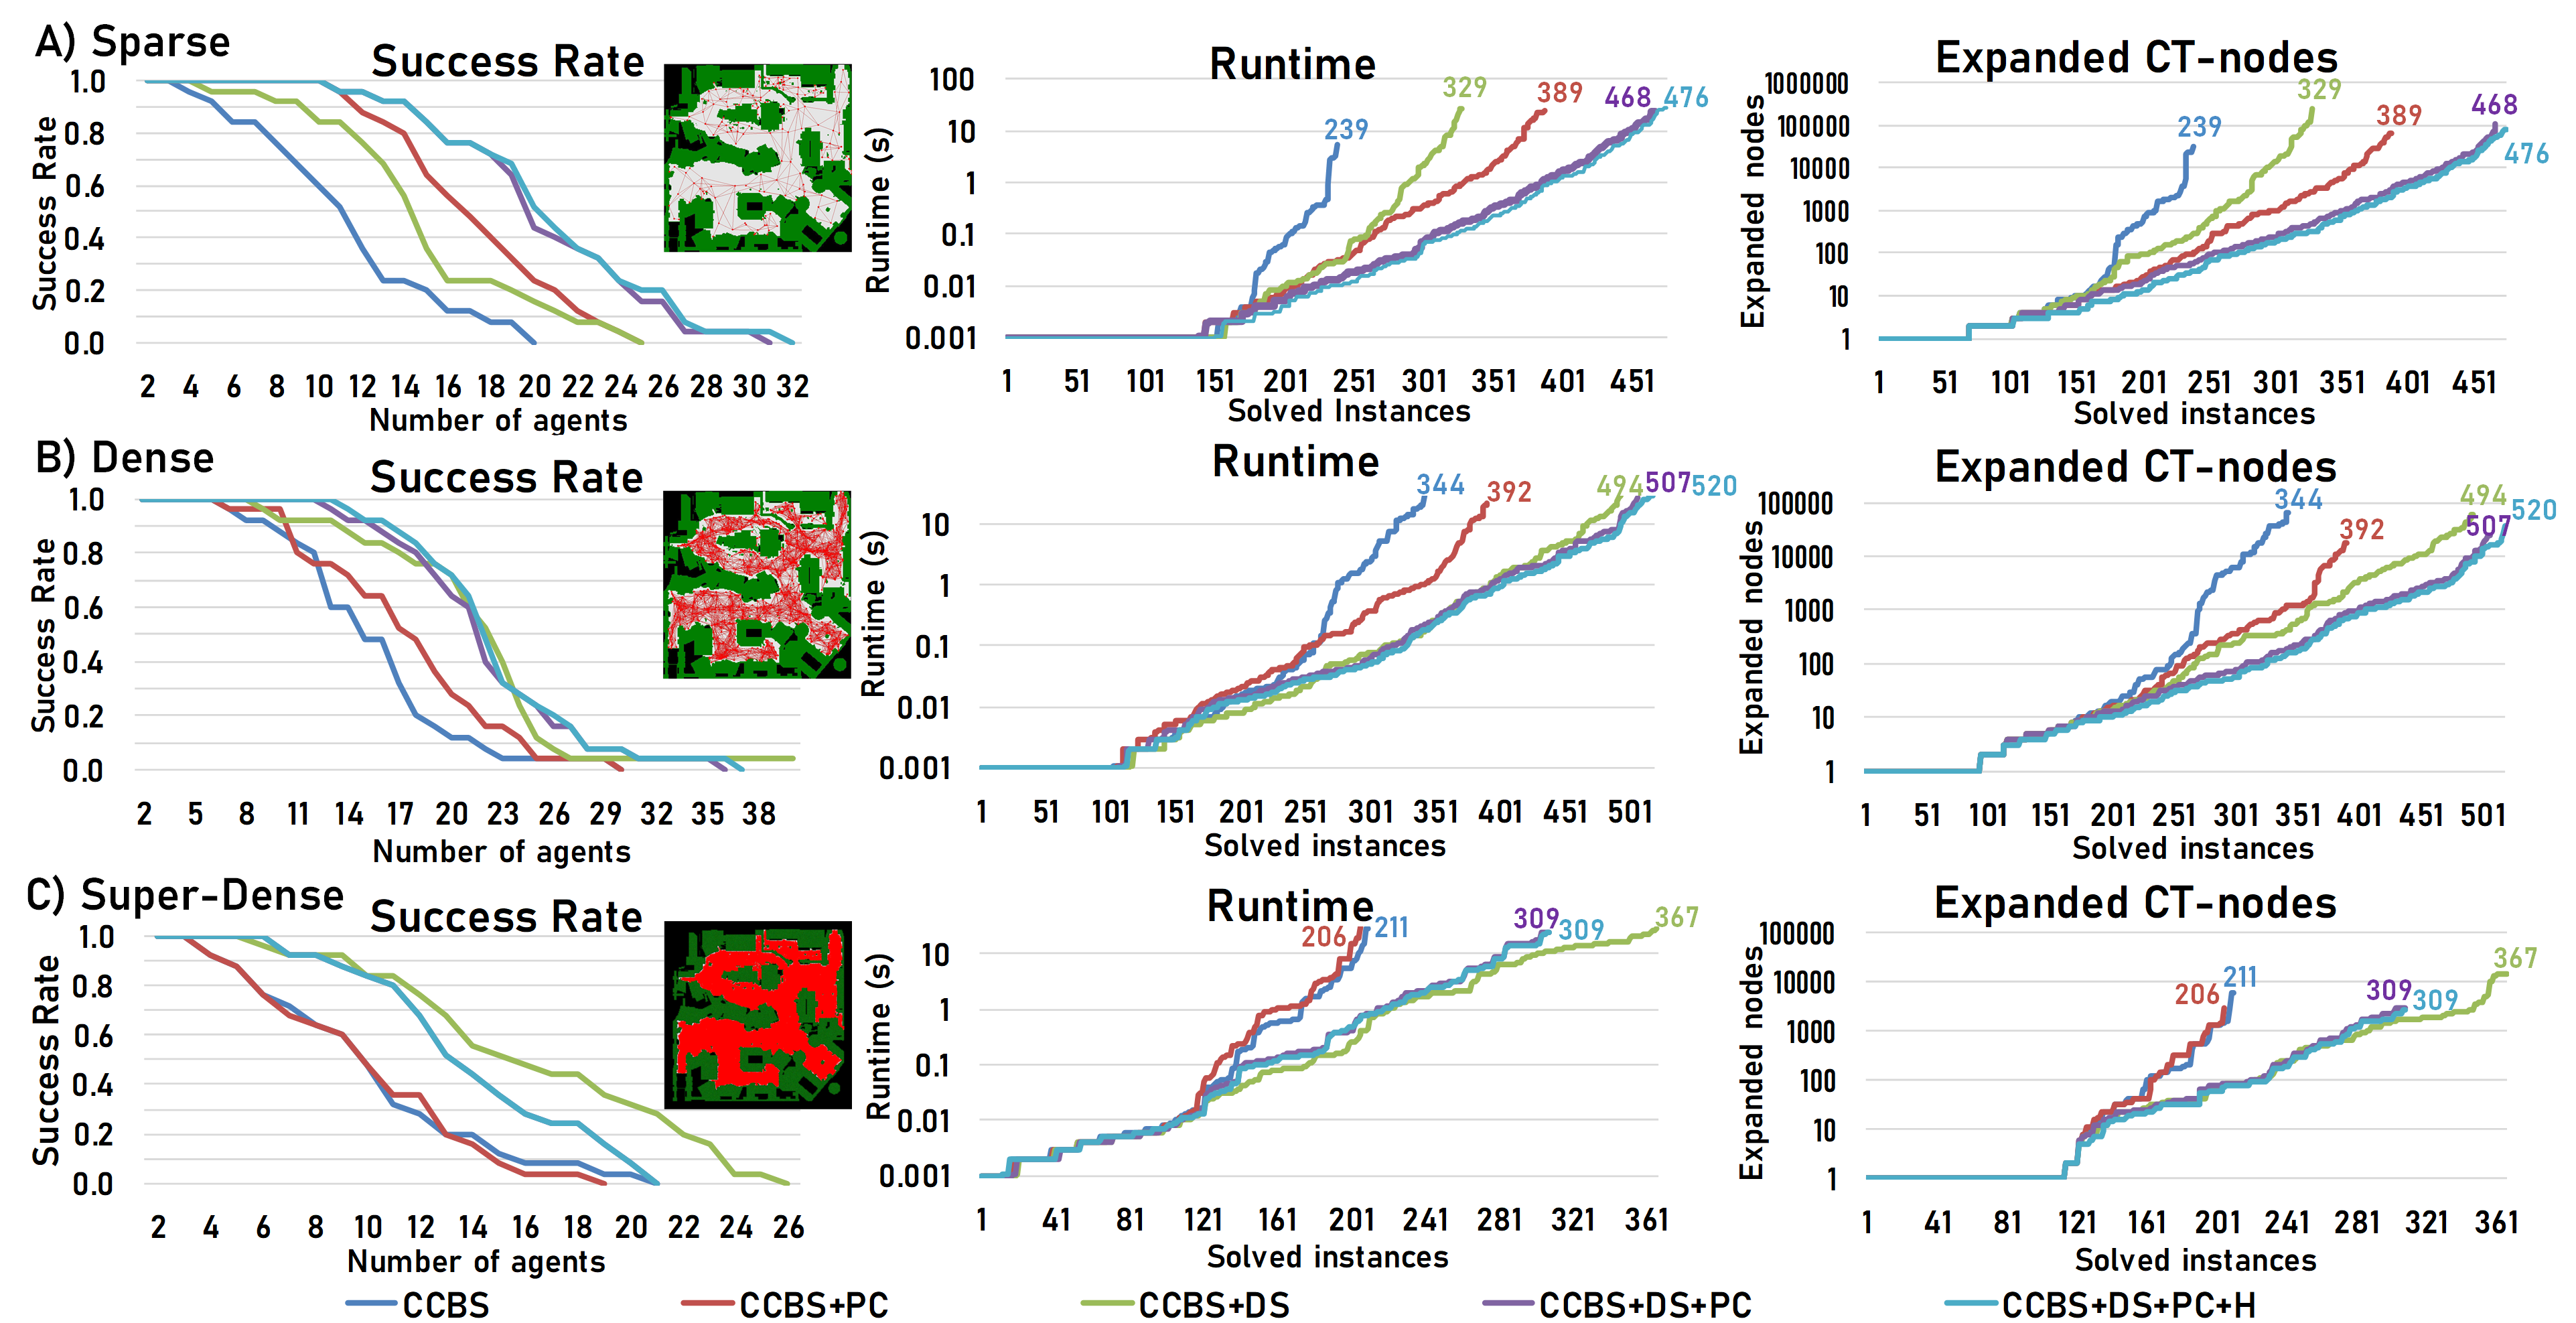
\includegraphics[width=\textwidth]{Roadmaps_results.png}
    \caption{Evaluation of different versions of CCBS on the sparse, dense, and super-dense roadmaps.}
    \label{figRoadmapsResults}
\end{figure*}

\begin{figure*}[t]
    \centering
    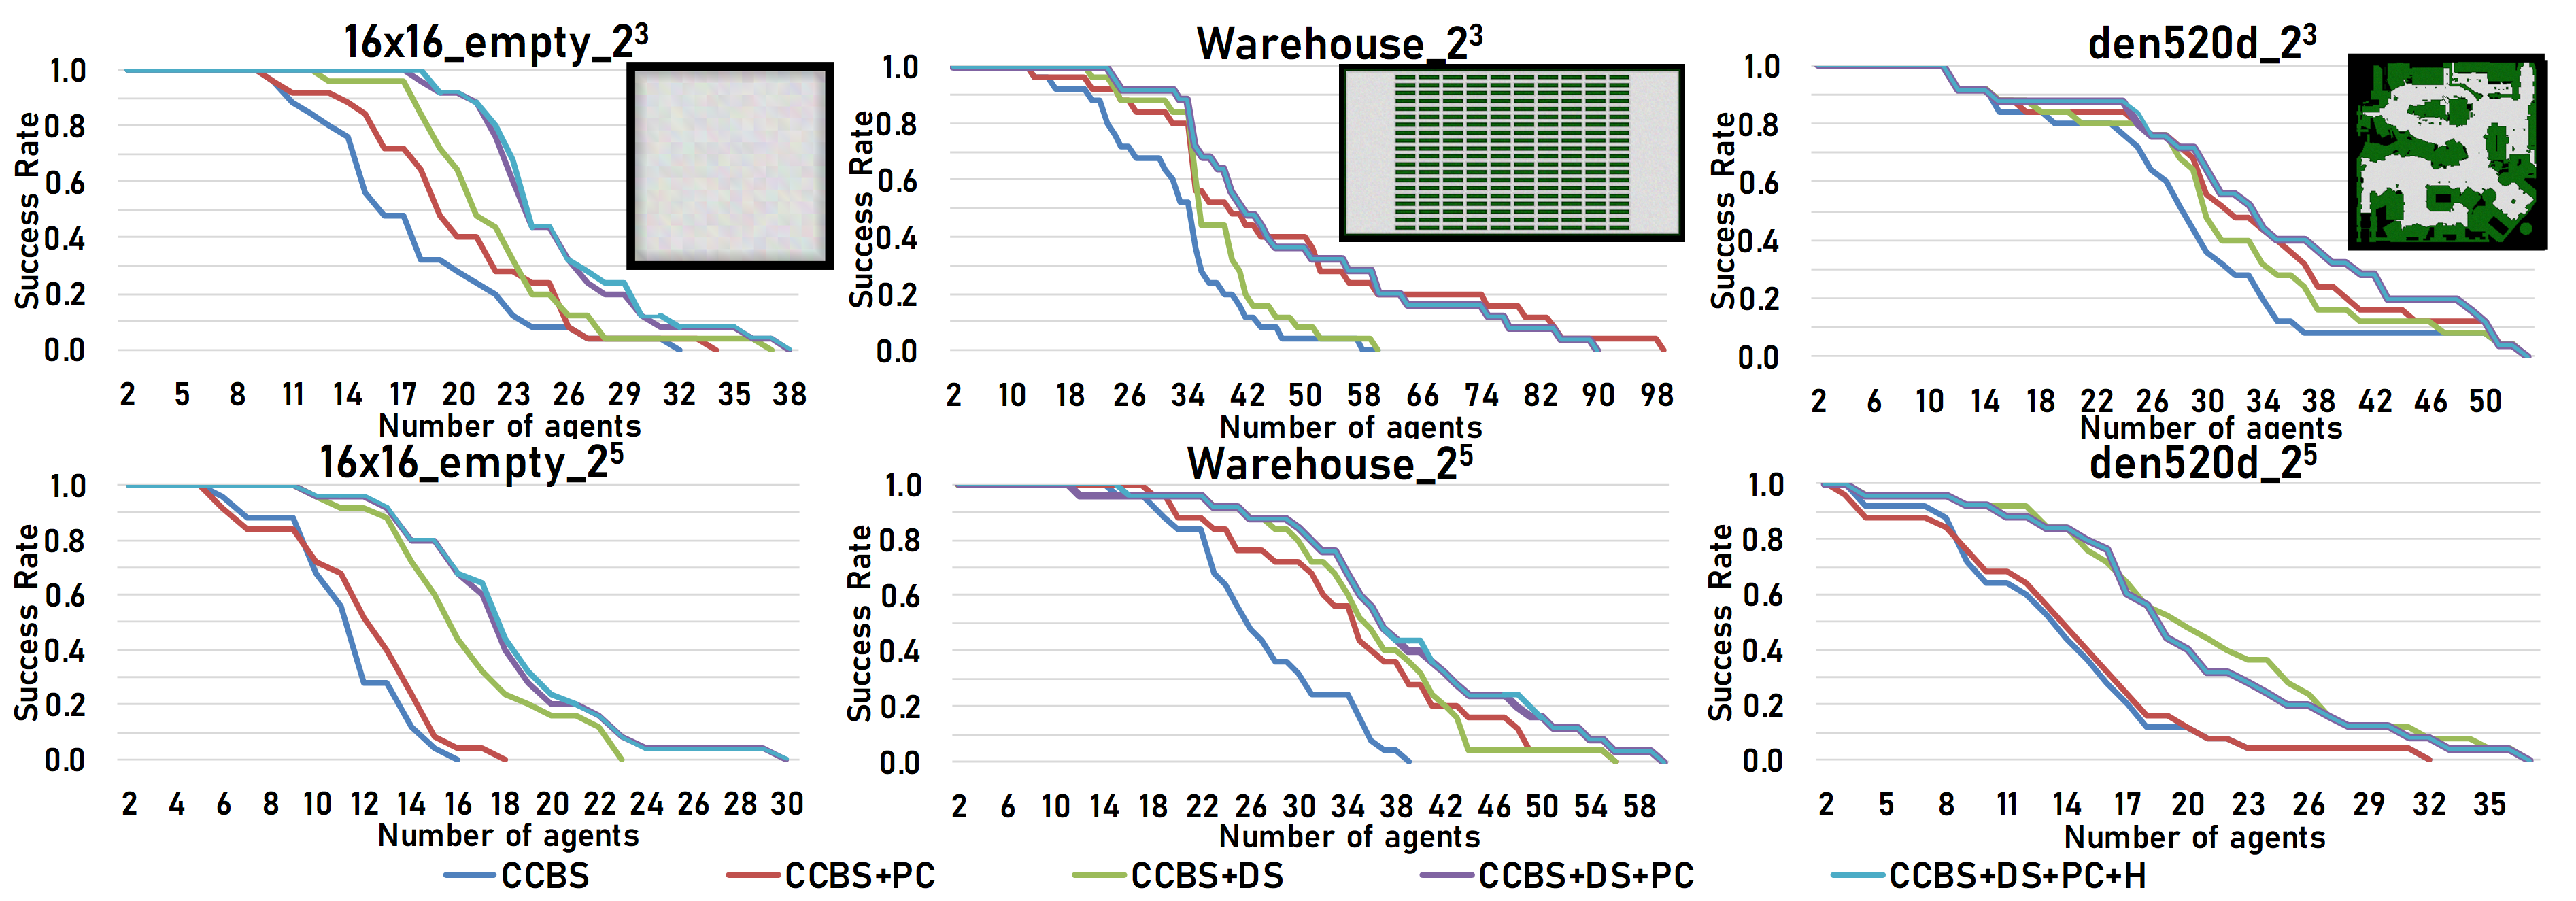
\includegraphics[width=\textwidth]{Grids_SR_all.png}
    \caption{Success rates of different versions of CCBS on different grids with $2^3$ and $2^5$-connectedness.}
    \label{figGridsResults}
\end{figure*}

We have incorporated all the \ccbs enhancements described so far and evaluated different versions of \ccbs in different \mapfr scenarios involving general graphs (roadmaps) and grids. 
Specifically, we evaluated the basic \ccbs, \ccbs with \pc (\ccbs+\pc), \ccbs with \ds (\ccbsds), 
\ccbs with both \ds and \pc (\ccbs+\ds+\pc), 
and \ccbs with all the improvements (\ccbs+\ds+\pc + H). 
In the conducted experiments all agents are assumed to be disk-shaped with radius equal to $\sqrt{2}/4$. 



In each run of the evaluated algorithm, we recorded the algorithm's runtime, the number of expanded \ct nodes, and whether the algorithm was able to find a solution under a time limit of 30 seconds or not. 
One of the primary evaluation metrics in our evaluation is the \emph{Success rate}, which is the ratio $N_{sol}/N_{all}$, where $N_{sol}$ is the number of instances the algorithm managed to solve under the imposed time cap and $N_{all}$ is the total number of instances. 

% homogeneous and represented as disks with radius equal to $\sqrt{2}/4$. %All agents move with equal constant speed. Inertial effects are neglected. roni: we say this already above
% For the sake of simplicity, we assume disk-shaped agents and define the \emph{location} of the agent as the center of this shape. % in this work. 



%Different versions of \ccbs are named as follows in the rest of the paper:
%1) \ccbs - baseline version without any enhancements;
%2) \ccbs+PC -  with \textbf{prioritizing conflicts};
%3) CCBS+DS - \ccbs with \textbf{disjoint splitting};
%4) CCBS+PC+DS - \ccbs that combines both \textbf{prioritizing conflicts} and \textbf{disjoint splitting};
%5) CCBS+PC+DS+H - the most modified version of CCBS that besides \textbf{prioritizing conflicts} and \textbf{disjoint splitting} also uses \textbf{high-level heuristic}.

\subsection{Implementation Details}

% As it was mentioned in the original paper on \ccbs~\cite{andreychuk2019multi} the 
Conflict detection in \mapfr is more involved than in classical \mapf and are more computationally intensive~\cite{andreychuk2019multi}. 
To compensate for that we have implemented the following approach to cache the intermediate conflict detection results and speed up the search. 
We detect all the conflicts in the root \ct node and store them with the node. 
After choosing a conflict and performing a split we copy all the conflicts to a successor node except the ones involving the agent that has to re-plan its path. 
After such re-planning newly introduced conflicts (if any) are added to the set of conflicts for that \ct node. 
To compute the \emph{cost impacts} of the conflicts for versions of \ccbs that use \pc or the high-level search heuristic $H$, we run the low-level search explicitly to resolve these conflicts and acquire the needed cost increase values. For versions of \ccbs without \pc, we picked the latest conflict out of all conflicts associated with the node. Our preliminary tests have showed that this ad-hoc strategy leads to better results when compared to choosing a conflict randomly or choosing the earliest conflict.
\roni{If we are stressed for space, we should remove this last bit about choosing the latest conflict.}


To speed-up the low-level search, we pre-compute a set of heuristics, $h_1$, ..., $h_n$ each of which estimates costs-to-go to a particular goal $g_n$. To compute $h_i$ we run Dijkstra's algorithm with $g_i$ as the source node. Indeed, such heuristics are more informative compared to e.g. Euclidean distance. 
When \ds is used, the low-level search performs multiple searches to achieve the landmarks created by the positive constraints. When searching for the intermediate goals associated with each landmarks, we implemented a Differential Heuristic (DH)~\cite{goldenberg2011compressed} that uses the pre-computed heuristics $h_1,\ldots, h_n$ as pivots. % (see the original paper on DH for more details). 



\subsection{Evaluation on the Roadmaps}

In the first set of experiments we have evaluated \ccbs on 3 different roadmaps, referred to here as \emph{sparse}, \emph{dense} and \emph{super-dense}. The sparse roadmap contains 158 nodes and 349 edges, the dense roadmap contains 878 nodes and 7,341 edges, and the super-dense roadmap contains 11,342 vertices and 263,533 edges. All of these graphs were automatically generated by applying a roadmap-generation tool from the Open Motion Planning Library (OMPL)~\cite{sucan2012ompl} on the the \texttt{den520d} map from the game Dragon Age Origin (DAO). This map is publicly available in the MovingAI \mapf benchmark~\cite{stern2019multi}. 
% We used a roadmap-generation tool from the Open Motion Planning Library (OMPL)~\cite{sucan2012ompl} to get the roadmaps. 

For each roadmap 25 different scenarios were generated. Each scenario is a list of start-goal vertices that were chosen randomly from the graph. 
\roni{Did you use your own scenarios or did you use the scenario files in the \mapf benchmark?} 
When testing we picked the first $n=2$ start-goal pairs from a scenario and create a \mapfr instance for $n$ agents. 
If the evaluated algorithm solved this instance within the 30 seconds time limit, we proceed to perform a new experiments by increasing $n$ by 1. This is repeated until the evaluated algorithm was not able to solve the instance in 30 seconds. We then proceed to the next scenario. 



The results are shown in Fig.\ref{figRoadmapsResults}. Consider first the success rate plots (left). \roni{Need to first highlight that everything is MUCH better than vanilla and give numbers}
The results show that the most advanced version of the algorithm, i.e. \ccbs+\pc+\ds+H, outperforms the competitors on sparse and dense roadmaps. 
However on the super-dense this is not the case. On this roadmap, \ccbs+\pc+\ds+H is dominated by \ccbs+\ds. 
Indeed, in this roadmap the \pc component is ineffective, as can be seen when comparing the basic \ccbs and \ccbs+\pc. 
We explain this behavior by observing that this roadmap has a very high branching factor in this map (every vertex has almost 50 neighbors on average). 
This helps to eliminate conflicts by finding an appropriate detour of nearly the same cost. As a result the cost impacts, which are computationally intensive to compute, are very low. Thus, they provide limited value in differentiate between conflicts and thus are not worthwhile. %. them while computing the cost impact is a computationally intensive routine involving low-level search.


% Note that both \pc and $H$ require computing the cost impacts, which is computationally intensive. 
% We conjecture that due to , they are 

% In fact, in this  is primarily due to the \pc component being ineffective, as can be seen when comparing the basic \ccbs and \ccbs+\pc. 
% due to to the very high branching factor in this map (every vertex has almost 50 neighbors on average). 
% This helps to eliminate conflicts by finding an appropriate detour of nearly the same cost. As a result the cost impacts, which are computationally intensive to compute, are very low. Thus, they provide limited value in differentiate between. them while computing the cost impact is a computationally intensive routine involving low-level search.

%As one can see, there is no a univocal version of CCBS that shows the best results. On sparse and dense roadmaps the best success rate has shown the CCBS+PC+DS+H version, while on the largest roadmap the best results has obtained the CCBS+DS version. Such behavior can be explained by the fact that PC enhancement on super-dense roadmap doesn't provide a positive benefit. There are two reasons of such behavior. Both of them are related to the large size of the graph and its high connectivity - every vertex has almost 50 neighbors on average. As a result, the algorithm requires a lot of time to calculate the cost increases associated with the conflicts, as the only way to find them - to replan the path with a new negative constraint associated with the conflict. Moreover, due to the high-connectedness of the graph there is always an alternative path that allows to satisfy the new constraint with almost equal cost. As a result the additional costs of all conflicts are very low and there is no much difference between them.

Next, consider the runtime and expanded \ct nodes plots in Figure~\ref{figRoadmapsResults}. 
These plots are built in the following fashion. 
Each data point $(x,y)$ on a plot says that an algorithm was able to solve $x$ problem instances within $y$ seconds/\ct nodes expansions. 
For example, on the dense roadmap \ccbs solved only 276 instances in less than 1 second, \ccbs+PC -- 340 instances, while \ccbs+\pc+\ds+H -- 404. In general, the closer the line to $x$-axis and the longer it is -- the better. The values at the end of the lines show the exact numbers of the solved instances. 

The general trends for runtime and high-level expansions are similar to the ones for success rate: \ccbs+\pc+\ds+H is the best on sparse and dense roadmaps and \ccbs+\ds -- on the super-dense one. The plots also provide a clear evidence that in some cases the most advanced versions of \ccbs are up to 2 orders of magnitude faster than vanilla \ccbs. \roni{Good sentence, we may want to mention this in the intro or abstract or both}



We also analyzed separately the impact of adding the high-level heuristic ($H$) on the instances that involve large numbers of \ct expansions. We took the results of 100 instances with the highest values of expanded \ct nodes solved by \ccbs+DS+PS and \ccbs+DS+PC+H averaged the number of expansions and compared them. The number of expansions for \ccbs+DS+PC+H was lower by 26.5\%, 21.6\% and 17.8\% for sparse, dense and super-dense roadmaps respectively. Thus, adding heuristic proved to be a valuable technique, especially for the hard instances involving large number of expansions.

\subsection{Evaluation on Grids}

% The second set of experiments we performed
% To assess the impact of the suggested enhancements of CCBS on grids, 
The second set of experiments we conducted was on 8-connected($2^3$) and 32-connected($2^5$) grids from the MovingAI \mapf benchmark~\cite{stern2019multi}. 
Specifically, we used a 16x16 empty grid (16x16\_empty), a warehouse-like grid (warehouse-10-20-10-2-2), and a grid representation of the den520d DAO map mentioned above. 
%All these maps and instances for them were taken from the MovingAI \mapf benchmark~\cite{stern2019multi}. 
Here we used the 25 scenario-files supplied by the \mapf benchmark for each grid. 
%Besides the mentioned above properties of the agents, the one needs to set the connectivity of the grid. In the conducted experiments we have evaluated 8-connected($2^3$) and 32-connected($2^5$) grids. 
The results of the second series of experiments are shown in Fig.\ref{figGridsResults}.


Here we can see that in almost all cases %except den520d grid with $2^5$-connectedness 
the best results were obtained by \ccbs with all our enhancements (\ccbs+\pc+\ds+H). 
%Notably, there were some scenarios on warehouse\_$2^3$ grid, where \ccbs+\pc solved more instances than \ccbs+\pc+\ds+H. % with more agents than CCBS+PC+DS or CCBS+PC+DS+H.
Comparing the results on grids with different connectedness, the one can notice the same trend as observed for roadmaps with respect to the benefit of \pc and \ds: increasing the branching factor makes \pc less effective and \ds more effective. %while \d Due to the increased amount of possible alternatives for the low-level planner, the benefit from PC in terms of success rate is much less on $2^5$-connected grids than on $2^3$-connected grids. In contrary, the benefit from DS is higher on high-connected grids. 
This benefit for \ds is explained by the fact that positive constraints help to reduce the branching factor by reducing the amount of possible alternative trajectories to one. Thus, higher branching factor means stronger pruning by positive constraints. 


%Both these versions have shown equal results and totally solved 1139 instances against 1111 solved by CCBS+PC on warehouse map. Talking about the high-level heuristic, its addition allowed to solve 8 more instances on 16x16\_empty map and only 1 more instance on den520d map.



%\roni{It is interesting that PC seems to be more effective in grids while DS is more effective for roadmaps. Would you agree? if so, maybe you have a nice explanation?}

% \begin{table}
% \centering
% \resizebox{0.8\columnwidth}{!}{
% \begin{tabular}{@{}lll|lll|lll@{}}
% \toprule
% \multicolumn{3}{l|}{16X16 Empty} & \multicolumn{3}{l|}{Warehouse} & \multicolumn{3}{l}{Den520} \\ \midrule
% $n$      & k=3     & k=5     & $n$     & k=3     & k=5    & $n$    & k=3    & k=5   \\ \midrule
% 10          & X       & X       & 40         & X       & X      & 10        & X      & X     \\
% 15          & X       & X       & 50         & X       & X      & 20        & X      & X     \\
% 20          & X       & X       & 60         & X       & X      & 30        & X      & X     \\
% 25          & X       & X       & 70         & X       & X      & 40        & X      & X     \\
% 30          & X       & X       & 80         & X       & X      & 50        & X      & X     \\ \bottomrule
% \end{tabular}
% }
% \caption{}
% \label{}
% \end{table}

\begin{table}
\resizebox{\columnwidth}{!}{
\begin{tabular}{| c | c c | c c | c c | c c |}
\hline
 & \multicolumn{2}{|c|}{PC} & \multicolumn{2}{c|}{DS}& \multicolumn{2}{c|}{PC+DS}& \multicolumn{2}{c|}{PC+DS+H}\\
& k=3 & k=5 & k=3 & k=5 & k=3 & k=5 & k=3 & k=5\\
\hline
16x16 & 33.1\% & 72.1\% & 13.97\% & 14.8\% & 6.7\% & 10.2\% & 5.6\% & 9.8\% \\
warehouse & 14.0\% & 15.7\% & 28.64\% & 23.7\% & 10.8\% & 18.4\% & 10.8\% & 14.3\% \\
den520d & 31.2\% & 100\% & 37.50\% & 67.7\% & 17.4\% & 76.4\% & 14.3\% & 67.1\% \\
\hline
\end{tabular}
}
\caption{The ratio of expanded CT-nodes between CCBS and its modifications on grids.}
\label{TableGridsExpansions}
\end{table}


Finally, calculated the ratios of expansions between the vanilla CCBS and the other versions
on the 100 instances in each grid that incured the highest number of \ct node expansions by the basic \ccbs and were solved by all \ccbs variants. 
% to evaluate the impact of different enhancements on the amount of expanded \ct nodes, we considered the 100 instances per each map that were solved by all versions and had the highest number of \ct node expansions by vanilla CCBS. 
% Further we have
The corresponding median values are presented in Table \ref{TableGridsExpansions}. As one can see, the least amount of expansions in all the cases requires the most advanced version, i.e. CCBS+PC+DS+H. It is also worth to note that in almost all the cases, additional connectivity of the grid makes all the enhancements less beneficial. The only case when this statement doesn't hold is the evaluation of CCBS+DS on warehouse grid. 


%\begin{table}
%\resizebox{0.8\columnwidth}{!}{
%\begin{tabular}{@{}llllllllll@{}}
%b         & b      & DS  & b   & PC  & b   & DS+PC & b   & DS+PC+H & b   \\
%b         & Agents & k=3 & k=5 & k=3 & k=5 & k=3   & k=5 & k=3     & k=5 \\
%16x16     & 10     & X   & X   & X   & X   & X     & X   & X       & X   \\
%X         & 15     & X   & X   & X   & X   & X     & X   & X       & X   \\
%X         & 20     & X   & X   & X   & X   & X     & X   & X       & X   \\
%X         & 25     & X   & X   & X   & X   & X     & X   & X       & X   \\
%X         & 30     & X   & X   & X   & X   & X     & X   & X       & X   \\
%Warehouse & 40     & X   & X   & X   & X   & X     & X   & X       & X   \\
%X         & 50     & X   & X   & X   & X   & X     & X   & X       & X   \\
%X         & 60     & X   & X   & X   & X   & X     & X   & X       & X   \\
%X         & 70     & X   & X   & X   & X   & X     & X   & X       & X   \\
%X         & 80     & X   & X   & X   & X   & X     & X   & X       & X   \\
%DAO       & 10     & X   & X   & X   & X   & X     & X   & X       & X   \\
%X         & 20     & X   & X   & X   & X   & X     & X   & X       & X   \\
%X         & 30     & X   & X   & X   & X   & X     & X   & X       & X   \\
%X         & 40     & X   & X   & X   & X   & X     & X   & X       & X   \\
%X         & 50     & X   & X   & X   & X   & X     & X   & X       & X  
%\end{tabular}
%}
%\end{table}

\section{Conclusions and Future Work}
In this work, we propose three improvements to \ccbs, an algorithm for finding optimal solutions to \mapfr problems in which time is continuous. 
The first \ccbs improvement we proposed, called \ds, changes how \ct nodes are expanded by introducing positive and negative constraints. 
To implement this improvement, we modified the \ccbs low-level search and applied a generalized version of \sipp multiple times with multiple start and goal nodes. 
The second \ccbs improvement we proposed, called \pc, prioritizes the conflicts to resolve by computing the cost of the solution that resolves them. 
The third \ccbs improvement we proposed is two admissible heuristics for the high-level search. 
In a comprehensive experimental evaluation, we observed that using these improvements, \ccbs can scale to solve much more problems than the basic \ccbs, solving in some cases almost twice as many agents. 
Allowing \ccbs to scale to larger problem is key to applying it to a wider range of real-world applications, e.g., in robotics, and also as a foundation for more generate \mapf settings in which the underlying graph is also changing rapidly. 

% %KONSTANTIN: I purposefully did not use acronym commands in abstract
% Conflict-Based Search (CBS) is a powerful algorithmic framework for optimally solving classical multi-agent path finding (MAPF) problems, where time is discretized into the time steps. 
% %If time is not discretized, the number of possible wait actions is uncountable. 
% Continuous-time CBS (CCBS) is a recently proposed version of CBS that guarantees optimal solutions without the need to discretize time. 
% However, the  scalability of CCBS is limited because it does not include any known improvements of CBS. 
% In this paper, we begin to close this gap and explore how to adapt successful CBS improvements, namely, prioritizing conflicts (PC), disjoint splitting (DS), and high-level heuristics, to the continuous time setting of CCBS. 
% %domain is not trivial as requires careful reasoning over the time intervals and the ways different time intervals interfere. 
% These adaptions are not trivial, and require careful handling of different types of constraints, applying a generalized version of the \acf{SIPP} algorithm, and extending the notion of cardinal conflicts.  
% % Moreover, the adaptions are applicable to other CBS-based algorithms that address have non-unit action costs. 
% We evaluate the effect of the suggested enhancements by running experiments both on general graphs and $2^k$-neighborhood grids. 
% CCBS with these improvements significantly outperforms vanilla CCBS, 
% solving problems with almost twice as many agents in some cases and 
% pushing the limits of multi-agent path finding in continuous-time domains. 
% Adding other enhancements. Introducing bounded-suboptimal versions of CCBS. Going towards ``fully-continuous'' MAPF problems.


\bibliography{mapf.bib}

\end{document}
